%% This is file `elsarticle-template-1-num.tex',
%%
%% Copyright 2009 Elsevier Ltd
%%
%% This file is part of the 'Elsarticle Bundle'.
%% ---------------------------------------------
%%
%% It may be distributed under the conditions of the LaTeX Project Public
%% License, either version 1.2 of this license or (at your option) any
%% later version.  The latest version of this license is in
%%    http://www.latex-project.org/lppl.txt
%% and version 1.2 or later is part of all distributions of LaTeX
%% version 1999/12/01 or later.
%%
%% The list of all files belonging to the 'Elsarticle Bundle' is
%% given in the file `manifest.txt'.
%%
%% Template article for Elsevier's document class `elsarticle'
%% with numbered style bibliographic references
%%
%% $Id: elsarticle-template-1-num.tex 149 2009-10-08 05:01:15Z rishi $
%% $URL: http://lenova.river-valley.com/svn/elsbst/trunk/elsarticle-template-1-num.tex $
%%

\documentclass[preprint,12pt]{elsarticle}

%% The amssymb package provides various useful mathematical symbols
\usepackage{amssymb}
%% The amsthm package provides extended theorem environments
%% para que haya environment proof
\usepackage{amsthm}

% necesario para align, aligned, gather, gathered, multline 
\usepackage{amsmath}

%para poder escribir pseudo codigo y nombres de algoritmos
\usepackage{clrscode}

\newtheorem{defn}{Definition}[section]
%\newcounter{defn} \numberwithin{defn}{section}
%\if@contnum
%\newtheorem{teo}[defn]{Theorem}
%\newtheorem{cor}[defn]{Corolary}
%\newtheorem{lema}[defn]{Lemma}
%\newtheorem{prop}[defn]{Proposition}
%\newtheorem{exmp}{Example}
%\newtheorem{remark}{Remark}
%\newtheorem{note}{Note}
%\else
%\newtheorem{teo}{Theorem}[section]
%\newtheorem{cor}{Corolary}[section]
%\newtheorem{lema}{Lemma}[section]
%\newtheorem{prop}{Proposition}[section]
%\newtheorem{exmp}{Example}[section]
%\newtheorem{remark}{Remark}[section]
%\newtheorem{note}{Note}[section]
%\fi

%Each of the functions above are a variation of the basic schema:

%\newtheorem{name}[counter]{Displayed Name}[orderby]


%para poder ocupar varias columnas
\usepackage{multicol}

%para poder dibujar grafos
\usepackage{tikz}
\usetikzlibrary{shapes.geometric}
\usetikzlibrary{decorations.markings}

%para poder agregar figuras que son .tex
\usepackage{standalone}

%para que no haya problemas con las tildes
\usepackage[utf8]{inputenc}

%% Use the option review to obtain double line spacing
%% \documentclass[preprint,review,12pt]{elsarticle}

%% Use the options 1p,twocolumn; 3p; 3p,twocolumn; 5p; or 5p,twocolumn
%% for a journal layout:
%% \documentclass[final,1p,times]{elsarticle}
%% \documentclass[final,1p,times,twocolumn]{elsarticle}
%% \documentclass[final,3p,times]{elsarticle}
%% \documentclass[final,3p,times,twocolumn]{elsarticle}
%% \documentclass[final,5p,times]{elsarticle}
%% \documentclass[final,5p,times,twocolumn]{elsarticle}

%% if you use PostScript figures in your article
%% use the graphics package for simple commands
%% \usepackage{graphics}
%% or use the graphicx package for more complicated commands
%% \usepackage{graphicx}
%% or use the epsfig package if you prefer to use the old commands
%% \usepackage{epsfig}


%% The lineno packages adds line numbers. Start line numbering with
%% \begin{linenumbers}, end it with \end{linenumbers}. Or switch it on
%% for the whole article with \linenumbers after \end{frontmatter}.
%% \usepackage{lineno}

%% natbib.sty is loaded by default. However, natbib options can be
%% provided with \biboptions{...} command. Following options are
%% valid:

%%   round  -  round parentheses are used (default)
%%   square -  square brackets are used   [option]
%%   curly  -  curly braces are used      {option}
%%   angle  -  angle brackets are used    <option>
%%   semicolon  -  multiple citations separated by semi-colon
%%   colon  - same as semicolon, an earlier confusion
%%   comma  -  separated by comma
%%   numbers-  selects numerical citations
%%   super  -  numerical citations as superscripts
%%   sort   -  sorts multiple citations according to order in ref. list
%%   sort&compress   -  like sort, but also compresses numerical citations
%%   compress - compresses without sorting
%%
%% \biboptions{comma,round}

% \biboptions{}

%% Miscelaneos
\newcommand{\STG}{\textit{STG}}
\newcommand{\GS}{\textit{GS}}

\newcommand{\cx}{\hat x}
\newcommand{\cc}{\hat c}
\newcommand{\ce}{\hat e}
\newcommand{\vx}{\vec{x}}
\newcommand{\x}{\vx}
\newcommand{\mult}{\cdot}


\journal{Advances in Applied Mathematics}

%\newcounter{dummy} \numberwithin{dummy}{section}
%\newtheorem{dummy}{dummy}[section]
%\newtheorem{teo}[dummy]{Theorem}[section]
%\newtheorem{lema}[dummy]{Lemma}[section]
%\newtheorem{cor}[dummy]{Corolary}
%\newtheorem{prop}[dummy]{Proposition}
%\newtheorem{exmp}{Example}
%\newtheorem{remark}{Remark}
%\newtheorem{note}{Note}

%\newproof{pf}{Proof}
%\newproof{pot}{Proof of Theorem \ref{thm2}}


 \newtheorem {teo}{Theorem}

\DeclareGraphicsRule{.tif}{png}{.png}{`convert #1 `dirname #1`/`basename #1 .tif`.png}

\newdefinition {remark}{Remark}

\newtheorem {definition}{Definition}

%\newtheorem {algorithm}{Algorithm}

\newtheorem {lema}[teo]{Lemma}

\newtheorem {cor}{Corollary}

\newtheorem{prop}{Proposition}

\newtheorem{exmp}{Example}

\newtheorem{note}{Note}





\begin{document}


\begin{frontmatter}

%% Title, authors and addresses

%% use the tnoteref command within \title for footnotes;
%% use the tnotetext command for the associated footnote;
%% use the fnref command within \author or \address for footnotes;
%% use the fntext command for the associated footnote;
%% use the corref command within \author for corresponding author footnotes;
%% use the cortext command for the associated footnote;
%% use the ead command for the email address,
%% and the form \ead[url] for the home page:
%%
%% \title{Title\tnoteref{label1}}
%% \tnotetext[label1]{}
%% \author{Name\corref{cor1}\fnref{label2}}
%% \ead{email address}
%% \ead[url]{home page}
%% \fntext[label2]{}
%% \cortext[cor1]{}
%% \address{Address\fnref{label3}}
%% \fntext[label3]{}

\title{Filters on disjunctive Boolean networks}

%% use optional labels to link authors explicitly to addresses:
%% \author[label1,label2]{<author name>}
%% \address[label1]{<address>}
%% \address[label2]{<address>}

\author{Francisco Plana}
\author[UCh]{Jorge Pérez}
\author[UAI]{Eric Goles}


\address[UAI]{Universidad Adolfo Ibáñez}
\address[UCh]{Universidad de Chile}


\begin{abstract}
%In this work we study the filters associated to block-sequential update schedules applied on Disjunctive Boolean networks. 
A filter is a procedure consisting in iteratively applying transformations to a Boolean network equiped with a specific updating scheme, such that fixed points of the initial network remain invariant. In this paper, we study the dynamics and complexity of filters applied on the class of disjunctive Boolean networks, which allow to study by means of the network digraph, and on block-sequential updating schemes.
%each of which simulates certain manner to update the network with parallel dynamics, producing a new network whose properties and dynamics can be related to the initial network. The main results of this work establish polynomial bounds for the time complexity of a filter. %We restrict our analysis to disjunctive Boolean networks, allowing us to concentrate only in the topology of the network. We focus also in block-sequential update schedules, which are a generalization of the parallel and sequential update schedules.
\end{abstract}

\begin{keyword}
Boolean networks \sep Regulatory networks \sep discrete dynamics \sep modeling 
%% keywords here, in the form: keyword \sep keyword

%% MSC codes here, in the form: \MSC code \sep code
%% or \MSC[2008] code \sep code (2000 is the default)

\end{keyword}

\end{frontmatter}

%%
%% Start line numbering here if you want
%%
% \linenumbers

%% main text

\section{Introduction}
\label{sec-intro}

%A Boolean network is a mathematical model proposed by Kauffman in the late $60$'s, initially to address the problem of spontaneous generation of order in complex systems \cite{kauffman}, \cite{kauffman_order}. A Boolean network consists of a finite set of Boolean functions, and is referred as a ``network'' since it can be represented as a digraph, where every node has a Boolean state that is the output of the respective Boolean function. The value returned by this function depends on the states of the neighbor nodes, and determines in turn, the evolution of the configuration of the network states over time. \par
%These models have acquired importance in last years as a tool to simulate the dynamics of gene regulatory networks, since the article published in 1998 by Mendoza \& Alvarez-Buylla \cite{mendoza_alvarez}, which studies floral morphogenesis of \textit{Arabidopsis thaliana}. Unlike other models based on differential equations, which exploit reaction kinetics in terms of rates and concentrations, Boolean networks do not require a large number of biochemical parameters difficult to estimate \cite{tyson_chen_novak}.\par %Although these networks are a simplification of the observed phenomenon -since they do not consider spatial aspects or continuous nature of gene and protein levels-, there are arguments to discretize the involved magnitudes: the functions that map the regulatory input signal (for example, stimulating protein level) to the response (for example, enzyme activity) can be approximated by functions similar to Heaviside step functions; several mechanisms \cite{sf}, \cite{ferrell} that would make this approximation valid have been suggested.\par
%In our setting, each function from the Boolean network is updated according to a deterministic ordering. For example, in the sequential case, functions are updated one after other one in some established order. In the parallel case, all network functions are updated at the same time. Or it can be a mixture of previous modes, which is called the block-sequential schedule, where some node groups are updated in parallel, and others in sequential way. Since the total number of network configurations is finite and the update mode is deterministic, the network states configuration converges, in a finite number of updates of the network from every possible initial state, to equilibrium points or attractors, where depending on the period length two behaviors are distinguished: fixed points, particular states of the network that remain constants over time, and limit cycles, sequences of network states that repeat over time.\par
%Several papers published in the last years have shown that fixed points of these networks may correspond, in many contexts, with observable biological states \cite{faure}, \cite{albert}, \cite{drosoph}. For example, the networks for the fission yeast cell cycle (the species \textit{Saccharomyces cerevisiae} \cite{yeast} and \textit{Schizosaccharomyces Pombe} \cite{pred_yeast}), whose dominant attractors correspond with observed stationary state G1. Or also in the network for the development of \textit{Arabidopsis thaliana} \cite{mendoza_alvarez}, the authors achieve to identify $4$ of its $6$ fixed points to the four specific tissues of the flower (sepals, petals, carpels and stamens). In the other hand, limit cycles do not have a clear biological meaning.\par  
%In this work we concentrate on studying certain aspects of attractors of Boolean networks, including computational aspects, characterizations, and so on, using the notion of ``filter''. A filter is a procedure consisting in iteratively applying transformations to a given network, each of these transformations simulates a certain way of updating a network under parallel dynamics. This produces finally a new network whose properties and dynamics can be related to the initial network. It has been shown that these filters can be very useful, as they deliver information efficiently about the fixed points of the input network (Goles and Salinas 2010 \cite{gol_sal}). In particular, the authors proved that the filtering procedure, under certain conditions over the initial network, outputs a Boolean network that preserves some attractors of the original network, the fixed points, and removes or filters out the limit cycles. %\par 
%By this reason, this procedure is named as ``Filter'', and it can be used to compute fixed points in polynomial time. This is a non-trivial property, since it is known that the general problem of existence of fixed points for Boolean networks is NP-Complete \cite{monfix_np}. %Thereby, the filters associated to sequential updates can be seen as part of a large set of algorithms developed in recent years to find Boolean network attractors: reduced order binary decision diagrams \cite{sync_async}, \cite{eff_2013}, scalar equation method \cite{find_cycl}, \cite{scal_eq}, based in power law \cite{imp_eff}, out-degree based gene ordering \cite{small_att}, SAT-based \cite{sat}, constraint programming \cite{log_an}. In general, existing algorithms were proposed for networks updated synchronously (in parallel), or asynchronously, where one node, selected randomly, is updated at each time. \par
\par  
%We restrict our analysis to disjunctive Boolean networks, allowing us to concentrate only in the topology of the network (see Section \ref{sec-disj-net}). These are networks whose Boolean functions only have disjunctions of variables. It is a good start point to restrict the goal of study in this sense, given the difficulties that may arise when functions defining the network become slightly more expressive. Potential complex or intractable behaviors in disjunctive networks may be evidence suggesting these difficulties.\par
%There are theorical works that have studied the phenomenon of distinct update schedules producing different dynamics in the same network \cite{par_ser}. 
% he lack of empirical knowledge about the order in which genetic regulations occur in biological networks, there makes no arguments to support the election of a more realistic iteration mode. However, community of biologists tend to agree that it is unlikely that genes involved in the same physiological function evolve in parallel \cite{gauges}. Other paper \cite{stabl_unst} affirms that a large fraction of attractors are an artifact produced by the parallel update, in the sense they are unstable to small perturbations or shifts of update events. By these reasons, it is of interest the study of Boolean network dynamics under more realistic and general update schedules than the parallel update. For this reason, we focus also in block-sequential update schedules (see Subsection \ref{subsec-updt-sched}), which are a generalization of the parallel and sequential update schedules. These schedules have been shown consistent with empirical data \cite{mendoza_alvarez}. \par%In fact, in the seminal work by Mendoza \& Alvarez-Buylla \cite{mendoza_alvarez}, a specific block-sequential update schedule was used in agreement to available experimental data regarding the activation order of gene groups.\par
%The structure of this work is as follows. Section \ref{sec-disj-net} explains some of the advantages and properties when considering disjunctive networks. Section \ref{sec-filt-conv} addresses the issue of the time required by the filtering procedure. Section \ref{sec-filt-cyc} investigates the condition over the initial network to ensure the remotion of limit cycles in the final network. Finally, Section \ref{sec-fix_p} studies when the filter attractor results to be a structural fixed point. The results obtained make use of positive matrix theory (see Subsection \ref{subsec-th-pos}).\par 

%The main results of this work establish polynomial bounds for the time complexity of a filter (Sections \ref{sec-mat-rep} and \ref{sec-filt-conv}), and conditions over the input network and schedule ensuring some properties in the output network including the removal of limit cycles (Sections \ref{sec-filt-cyc} and \ref{sec-fix_p}). The polynomial time for computing a filter (Theorem \ref{el_mas}) is a critical issue if the filter is thought of as an algorithm to find Boolean network attractors. This bound is derived from a general bound for the converge time to attractors in disjunctive Boolean networks (Theorem \ref{mainteo}). However, there are some cases in which the time for computing a filter could grow even super-polynomially; this situation is adressed in Theorem \ref{teo-superpol}. This intractable behavior appears when the filtering procedure converges to a set called the filter attractor that results to have a super-polynomial size. This behavior can be avoided, for example, when the filter attractor is a structural fixed point, that is, the filter attractor is a set formed by only one network. Theorem \ref{main-fp} establishes a condition on the input network that ensures that the filter attractor is a structural fixed point. In the other hand, Theorem \ref{filt} establishes a condition on the input network that ensures that the networks in the filter attractor do not have limit cycles when updated with the parallel schedule. The results obtained make use of positive matrix theory (see Subsection \ref{subsec-th-pos}).


\section{Definitions and theoretical framework}\label{defini}

%\subsection{Preliminaries}
%A \textit{digraph} (or \textit{directed graph}) $D=(V,A)$ consists of a finite set $V$ of elements called \textit{nodes} (or \textit{vertices}) and a prescribed set $A$ of ordered pairs of (not necessarily distinct) vertices of $V$. Every ordered pair $\alpha=(a,b)$ of vertices $a$ and $b$ in $A$ is called an \textit{arc} (or \textit{directed edge}) of the digraph $D$. %For the arc $\alpha=(a,b)$, the vertices $a$ and $b$ are called the \textit{endpoints} of $\alpha$, $a$ is called the \textit{initial vertex} and $b$ is called the \textit{terminal vertex}; also, it is said that vertex $a$ \textit{is incident to} vertex $b$. The vertex set of $D$ is referred to as $V(D)$, and its arc set as $A(D)$.\par
%A \textit{subdigraph} of $D$ is a digraph $D^{\prime}=(V^{\prime},A^{\prime})$ where $V^{\prime}\subseteq V$ and $A^{\prime}\subseteq (V^{\prime}\times V^{\prime})\cap A$. We write $D^{\prime}\subseteq D$. For a digraph $D=(V,A)$ and a set $V^{\prime}\subseteq V$, we define the subdigraph \textit{induced in }$D$ \textit{ by } $V^{\prime}$, which we denote as $D(V^{\prime})$, as the digraph whose vertex set is $V^{\prime}$, and its arc set is $(V^{\prime}\times V^{\prime}) \cap A$.\par
%For a digraph $D=(V,A)$, it is defined the \textit{transpose} (or \textit{reverse}) of $D$, which we will denote as $D^T$, as the digraph having the same vertex set $V$, and whose arcs are reversed with respect to the corresponding arcs of $A$, that is, $D^T=(V,A^T)$, where $A^T=\{(u,v)|(v,u)\in A\}$.\par 
%For a digraph $D=(V,A)$, it is defined the \textit{in-neighborhood} $N_D^-(i)$ of a node $i \in V$, as the set of incident vertices to $i$: $N_D^-(i)=\{j\in V | (j,i)\in A\}$. The \textit{in-degree} of $i$ is the cardinal of this set, denoted as $deg_D^-(i)$ ($deg_D^-(i)=|N_D^-(i)|$). The \textit{out-neighborhood} $N_D^+(i)$ of a node $i \in V$, is defined as the set of vertices at which $i$ is incident: $N_D^+(i)=\{j\in V | (i,j)\in A\}$. The \textit{out-degree} of $i$ is the cardinal of this set, denoted as $deg_D^+(i)$ ($deg_D^+(i)=|N_D^+(i)|$).\par 
%A \textit{directed walk} from vertex $v_0$ to vertex $v_m$ in a digraph $D$ is a sequence of vertices $v_0,v_1,\ldots,v_m$ of $V(D)$ such that $(v_k,v_{k+1}) \in A(D)$ for all $k=0,\ldots,m-1$. We say that a walk $v_0,v_1,\ldots,v_m$ has \textit{length} equal to $m$. A \textit{directed path} (or \textit{directed chain}) $v_0,v_1,\ldots,v_m$ is a directed walk with no repeated vertices, except perhaps $v_0$ and $v_m$. A \textit{closed walk} or \textit{circuit} is a directed walk $v_0,v_1,\ldots,v_m$ where $v_0=v_m$. A \textit{closed path}, \textit{simple circuit} or \textit{cycle} is a directed path $v_0,v_1,\ldots,v_m$ where $v_0=v_m$. A \textit{loop} is a cycle of length equal to $1$.\par
%Two vertices $a$ and $b$ are called \textit{strongly connected} provided there are directed walks from $a$ to $b$ and from $b$ to $a$. A vertex is regarded as trivially strongly connected to itself. %Defined in this way, strong connectivity is an equivalence relation: reflexive, symmetric and transitive. Hence strong connectivity yields a partition $(V_i)_{i=1}^{\mathcal{C}}$ of the vertex set of digraph $D$. The subdigraphs $D(V_1), D(V_2),\ldots,D(V_{\mathcal{C}})$ induced in $D$ by each equivalence class are called the \textit{ strongly connected components} (s.c.c.'s) of $D$. A digraph $D$ is \textit{strongly connected } if it has exactly one strongly connected component.\par
%Let $D$ be a digraph, and let $D(V_1), D(V_2),\ldots,D(V_{\mathcal{C}})$ the strongly connected components of $D$. Let $D^{*}$ be the digraph whose vertices are the sets $V_1, V_2,\ldots,V_{\mathcal{C}}$ in which there is an arc from $V_i$ to $V_j$ if and only if $i\neq j$ and there is an arc in $D$ from some vertex in $V_i$ to some vertex in $V_j$. The digraph $D^{*}$ is the \textit{condensation digraph} of $D$. It is not difficult to prove that $D^{*}$ does not have loops or closed directed walks, %(Lemma 3.2.2 in \cite{mat_book}), 
%therefore $D^{*}$ is a \textit{directed acyclic graph} (DAG) -that is, a directed graph with no directed cycles- and consequently admits a \textit{topological sort}, which is an ordering of its vertices such that for every arc, the initial vertex comes before the terminal vertex in the ordering.\par
%A \textit{graph} (or \textit{undirected graph}) $G=(V,E)$ consists of a finite set $V$ of elements called \textit{nodes} (or \textit{vertices}) and a prescribed set $E$ of $2$-element subsets of $V$ called \textit{edges} or \textit{lines}. For undirected graphs we can define \textit{walks}, \textit{paths}, \textit{circuits} and \textit{cycles} similarly to what was done for digraphs. We say an undirected graph $G=(V,E)$ is \textit{connected} if there is a path in $G$ between every pair of vertices in $V$.\par
%For a directed graph $D=(V,A)$ we can define the \textit{underlying graph} of $D$ as the undirected graph $G_D=(V,E_D)$, where $E_D=\{\{v,w\}|(v,w)\in A\vee (w,v) \in A\}$. We say that a digraph $D$ is \textit{weakly connected} if its underlying graph is connected.\par
%Finally, we will refer to some of the basic operations of Boolean algebra as follows: the conjunction (AND) of variables $x$ and $y$ is denoted as $x\wedge y$, and it satisfies $x\wedge y=1$ if and only if $x=y=1$. The disjunction (OR) of $x$ and $y$, denoted as $x\vee y$, meets that $x\vee y=0$ if and only if $x=y=0$. The negation (NOT), denoted as $\neg x$, is defined as follows: $\neg x=1$ if and only if $x=0$.    

%\subsection{Boolean networks}
%This section follows conceptualizations presented in \cite{disj} and \cite{gol_sal}. A 

A \textit{Boolean network} \textit{of size} $n$ is %defined by a \textit{global transition function}
a function $F:\{0,1\}^n\rightarrow\{0,1\}^n$, where $F(\vec{x})=(f_1(\vec{x}),\cdots,f_n(\vec{x}))$. For each $i \in \{1,\ldots,n\}$, $f_i:\{0,1\}^n\rightarrow\{0,1\}$ is called the $i-$th \textit{local transition function}. %The vector $\vec{x} \in \{0,1\}^n$ taken as argument by these functions is called vector of \textit{network configurations} or \textit{states}. %The intuition behind is, if current configuration of the network is $\vec{x}$, after updating node $i$ its new state is given by $f_i(\vec{x})$. 
We define the \textit{digraph associated to }$F$ as $D^F=(V,A)$, where %\begin{itemize}
%\item $V=\{1,\cdots,n\}$
%\item
$V=\{1,\cdots,n\}$ and $(i,j) \in A$ iff there exists some $\vec{x} \in \{0,1\}^n$ such that
%\begin{align*}
$$f_j(x_1,\cdots,x_{i-1},0,x_{i+1},\cdots,x_n)\neq \\f_j(x_1,\cdots,x_{i-1},1,x_{i+1},\cdots,x_n)$$
%\end{align*}
%\end{itemize}
%The intuition from the last definition is given by the fact that each node represents one component from the network state vector. So, there is an arc $(i,j)$ starting from node $i$ and ending on $j$, if function $f_j$ (or in other words, the component $j$ of network state vector after updating its value) depends on component $i$ from the current configuration vector. %As a consequence of this, the nodes without incident arcs are those corresponding to variables having a constant value, that is, those nodes $j$ such that $$f_j(\vec{x})=1 \quad\forall\vec{x} \in \{0,1\}^n \quad\text{ or } \quad f_j(\vec{x})=0 \quad\forall\vec{x} \in \{0,1\}^n $$

%Notice that a variable having a dependency on itself is represented in the graph as a \text{loop}: a cycle of length equal to one, connecting a node to itself. 
%Observe that the digraph associated to some Boolean network displays only dependencies existing between nodes, but without additional information the global transition function cannot be recovered from the associated digraph.    

%\begin{exmp}\label{ej-1st} 
%A Boolean network $N_F$ with its respective associated digraph is the following:
%\begin{multicols}{2}
%\begin{equation*}
%\begin{aligned}
%N_F:\\
%f_1(\vec{x})=&x_4\\
%f_2(\vec{x})=&x_1 \lor \lnot x_4\\
%f_3(\vec{x})=&x_2 \land x_3\\
%f_4(\vec{x})=&x_3 \land x_5\\
%f_5(\vec{x})=&\lnot x_2
%\end{aligned}
%\end{equation*}
%\begin{center}
%\documentclass{standalone}

\usepackage{tikz}

\usetikzlibrary{shapes.geometric}
\begin{document}
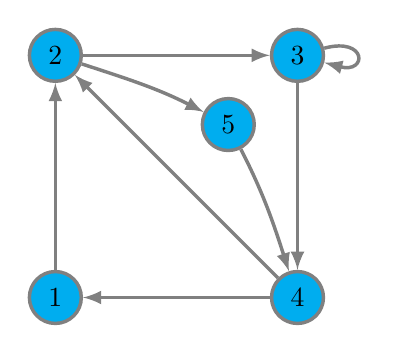
\begin{tikzpicture}
[every node/.style={inner sep=0pt}]
\node (2) [circle, minimum size=18.75pt, fill=cyan, line width=1.25pt, draw=gray] at (50.0pt, -25.0pt) {\textcolor{black}{2}};
\node (5) [circle, minimum size=18.75pt, fill=cyan, line width=1.25pt, draw=gray] at (112.5pt, -50.0pt) {\textcolor{black}{5}};
\node (1) [circle, minimum size=18.75pt, fill=cyan, line width=1.25pt, draw=gray] at (50.0pt, -112.5pt) {\textcolor{black}{1}};
\node (4) [circle, minimum size=18.75pt, fill=cyan, line width=1.25pt, draw=gray] at (137.5pt, -112.5pt) {\textcolor{black}{4}};
\node (3) [circle, minimum size=18.75pt, fill=cyan, line width=1.25pt, draw=gray] at (137.5pt, -25.0pt) {\textcolor{black}{3}};
\draw [line width=1.25, ->, >=latex, color=gray] (1) to  (2);
\draw [line width=1.25, ->, >=latex, color=gray] (2) to  (3);
\draw [line width=1.25, ->, >=latex, color=gray] (3) to  (4);
\draw [line width=1.25, ->, >=latex, color=gray, loop right] (3) to (3);
\draw [line width=1.25, ->, >=latex, color=gray] (4) to  (1);
\draw [line width=1.25, ->, >=latex, color=gray] (4) to  (2);
\draw [line width=1.25, ->, >=latex, color=gray] (2) to  [in=153, out=342] (5);
\draw [line width=1.25, ->, >=latex, color=gray] (5) to  [in=108, out=297] (4);
\end{tikzpicture}
\end{document}

%\end{center}
%\end{multicols}
%\end{exmp}

%\subsection{Dynamics of block-sequential update schedules}\label{subsec-updt-sched}

In order to introduce dynamics a Boolean network can be updated following a % we will consider an object called 
\textit{block-sequential update scheme}, defined as an ordered partition $\{B_0, ... B_{p}\}$ of $V$, with $p \leq |V|-1$, %where the set $B_j$ is referred as the $j-$th \textit{block}, 
or equivalently, by an \textit{update function} $s:V\rightarrow \{0,\ldots,p\}$ such that for each $i \in V$, $s(i)$ corresponds to the unique instant at which node $i$ is updated during one update sequence. Thus, for $j=0,\ldots,p$, $B_j=s^{-1}(\{j\})$. Each of the sets from the ordered partition is called as \textit{block}. %The semantics of the dynamics is as follows: a transition from any network configuration to another, is obtained after 
One iteration of the network consists in a complete update sequence, where the first nodes to be updated are those in the first block $B_0$, then the nodes in $B_1$, and so on up to the last block $B_{p}$. %This means that for each $i \in V$, $s(i)$ corresponds to the unique instant at which node $i$ is updated during one update sequence. 
If there is a unique block, i.e. $B_0=V$ we get the \textit{parallel} or \textit{synchronous} schedule, %usually 
notated as $\pi$. If we have $B_{j}=\{\sigma(j)\}$, where $\sigma$ is a permutation of $V$, we have a \textit{sequential} schedule.\par
Formally, for a Boolean network $F$ of size $n$ and a block-sequential schedule $s$, the dynamics is represented via the \textit{State Transition Graph} $\STG(F,s)=(H,T)$, where $H=\{0,1\}^n$ and $(\vec{x},\vec{y}) \in T$ if and only if $\vec{y}=F_s(\vec{x})$, where $F_s:\{0,1\}^n\rightarrow\{0,1\}^n$ is a function that outputs the new network configuration after a complete update sequence according to $s$. %Hence, arcs from $\STG(F,S)$ represent state transitions of network $F$ under one update with $S$. 
It is apparent that $F_s$ simulates in parallel the dynamics of $F$ under updating with $s$, that is, %in the sense that, if we call the parallel schedule as $\pi$, we have that
$$\STG(F,s)=\STG(F_s,\pi)$$


%Now we can define the \textit{global transition function of a network with update schedule} $S$, as the function $F_S:\{0,1\}^n\rightarrow\{0,1\}^n$ that outputs the new network configuration after a whole update sequence: $$F_S(\cdot)=F_{[B_{m-1}]} \circ\cdots\circ F_{[B_1]}\circ F_{[B_0]}(\cdot)$$
%For a Boolean network $F(\cdot)=(f_1(\cdot),\cdots,f_n(\cdot))$, updated with a block-sequential update schedule $S$ (and respective update function $s$) it is defined, for a node $i \in V$, the \textit{local transition function }$f_i^S$\textit{ relative to }$S$ as the $i-$th component function of $F_S$, that is
%$$F_S(\cdot)=(f_1^S(\cdot),\cdots,f_n^S(\cdot))$$
%The function $f_i^s(\cdot)$ corresponds to the state that node $i$ has once it has been updated during one update sequence and its update in the next update sequence. %Recall that for block-sequential update schedules, each node is updated only once during one update sequence. 

%as well as an initial condition given by $\vec{x}\in\{0,1\}^n$.
%A complete update sequence, 
%The network is updated following one by one the set of the partition. I.e. to update $I_{l}$ we consider the new state of every site in previous partition and the old state of partitions $I_{j}$, for $j\ge l$. 

%see Boolean networks as dynamical systems, an updating procedure of the network must be specified. Let $F:\{0,1\}^n\rightarrow\{0,1\}^n$ be a Boolean network and $D_F=(V,A)$ be the associated digraph, where we will use the next convention: $V=\{1,\ldots,n\}$. We define a \textit{block-sequential update schedule} $S$ by an \textit{update function} $s:V\rightarrow \{0,\ldots,n-1\}$, such that for each $i \in V$, $s(i)$ corresponds to the unique instant at which node $i$ is updated during one update sequence. A schedule $S$ is represented either by an \textit{update sequence} given by the sequence of sets $B_0,B_1,\ldots,B_{m-1}$, such that $m\leq n=|V|$ is the number of update instants of the sequence, and for each $j \in \{0,\ldots,m-1\}$, $B_j\subseteq V$, which will be referred as the \textit{$j-$th block}, refers to the set of nodes updated at instant $j$ of the update sequence. Notice that the update function and the update sequence of a schedule are indeed equivalent representations, since it holds that:
%$$B_j=\{k \in V| s(k)=j\}=s^{-1}(\{j\})$$
%Given this equivalence between these two representations, we will refer to a update schedule as a function or as a sequence of blocks interchangeably. %When there is no confusion about what schedule is referred, we will simply write $B_j$ instead of $B_j^S$, and $s$ instead of $s_S$. %A notation frequently used is to write the nodes belonging to one update block enclosed by a pair of parentheses, as can be seen in the next example.
%\begin{exmp}\label{first} 
%Let $V=\{1,2,3,4\}$ be the set of nodes of the digraph $G$ associated to a Boolean network $N_F$, and let $s:V\rightarrow\mathcal{P}(\{0,1,2,3\})$ the following update function: $s(1)=\phi$, $s(2)=\{0\}$, $s(3)=\{0,2\}$, $s(4)=\{1\}$. A more convenient notation for this schedule is to write its update sequence $(2,3)(4)(3)$, where nodes updated at the same time belong to some update block and are written in brackets; also the blocks are displayed in increasing order according the update instant.
%\end{exmp}  
%Notice that, in an arbitrary update schedule with update function $s$, some nodes could never be updated (a node $j$ verifying $|s(j)|=0$), while others could be updated more than once during one update sequence (a node $j$ verifying $|s(j)|>1$). In this work, an important definition will be that of \textit{block-sequential} update schedules: these are schedules where each node is updated exactly once during one update sequence, that is, for every $i \in V$, it holds that $|s(i)|=1$. For a block-sequential update schedule, since for each node $i \in V$ the set $s(i)$ results to be a singleton, we can compare update instants with the usual order in $\mathbb{N}$: we say the node $i$ is updated after node $j$ if $s(j)<s(i)$. Also, for a block-sequential update schedule $S$, the update function results to be $s:V\rightarrow \{0,\ldots,n-1\}$, %(the update function in general is defined as $s:V\rightarrow \mathcal{P}(\{0,\ldots,n-1\})$) the number of update instants verifies $m\leq n=|V|$, and 
%Since each node is updated only once, the set of blocks $(B_{\ell})_{\ell=0}^{m-1}$ is a partition of the set of nodes $V$. Two important block-sequential update schedules are the following:
%\begin{itemize}
%\item The \textit{parallel} schedule, usually denoted as $\pi$, is a schedule where %in which all the nodes of the network are updated at the same time. Therefore, in the parallel schedule 
%$there is just one block $B_0^{\pi}=V$.
%\item A \textit{sequential} schedule $S^{\prime}$ is that in which %one node is updated at every instant, that is, 
%for every $t < m$, $|B_t^{S^{\prime}}|=1$, and necessarily $m = |V|$. %is the number of blocks of $S^{\prime}$. Necessarily for these schedules, if $n$ is the number of nodes of the network, then $m=n$. 
%It can be assumed, without loss of generality (via a graph isomorphism), that the sequential schedule $S^{\prime}$ is the update function $s(i)=i-1$, for all $i \in V$.%corresponds to the fixed permutation $(1)(2)\cdots(n)$. 
%\end{itemize}

%\subsection{Dynamics of Boolean networks}

%Given a Boolean network $F(\cdot)=(f_1(\cdot),\cdots,f_n(\cdot))$ %$F$ of size $n$ with global transition function $F$ and local transition functions $(f_i)_{i=1}^n$ (that is, for each $\vec{x} \in \{0,1\}^n$, it holds that $F(\vec{x})=(f_1(\vec{x}),\cdots,f_n(\vec{x}))$), 
%and some update schedule $S$ with blocks $(B_{\ell})_{\ell=0}^{m-1}$, we want to formalize the notion of network dynamics. For this, it is defined the \textit{State Transition Graph} $\STG(F,S)=(V,A)$, where $V=\{0,1\}^n$ and $(\vec{x},\vec{y}) \in A$ if and only if $\vec{y}=F_{[B_{m-1}]} \circ\cdots\circ F_{[B_1]}\circ F_{[B_0]}(\vec{x})$, where 

%$$F_{[B_{\ell}]}(\vec{x})_i=\left\{\begin{array}{rl}f_i(\vec{x}) & i \in B_{\ell},\\x_i & \mbox{otherwise}\end{array}\right.$$ 

%$F_{[B_{\ell}]}(\cdot)$ is called the \textit{transition function with respect to the block }$B_{\ell} \subseteq V$ \textit{of nodes updated in parallel}. %The intuition of $\STG(F,S)$ is that arcs represent configuration or state transitions, from any possible state to the state obtained after a complete update sequence, where the first nodes to be updated are those in the first block $B_0$, then the nodes in $B_1$, and so on up to the last block $B_{m-1}$.\par
%Now we can define the \textit{global transition function of a network with update schedule} $S$, as the function $F_S:\{0,1\}^n\rightarrow\{0,1\}^n$ that outputs the new network configuration after a whole update sequence: $$F_S(\cdot)=F_{[B_{m-1}]} \circ\cdots\circ F_{[B_1]}\circ F_{[B_0]}(\cdot)$$ 

%\begin{exmp}\label{ex-net-updt}
%Let $N_F$ be the Boolean network of size $4$ and global transition function $F$, given by transition functions $f_1(\vec{x})=x_4$, $f_2(\vec{x})=x_1 \vee x_4$, $f_3(\vec{x})=x_1 \wedge x_2$ and $f_4(\vec{x})=x_3$, and let $S$ be the block-sequential schedule given by blocks $B_0=\{2,3\}$, $B_1=\{1,4\}$. If we start from state vector $\vec{y}=(0,1,0,1)$, to get the transition obtained after a complete update sequence with $S$, we first compute the vector $F_{[B_0]}(\vec{y})=(0,0\vee1,0\wedge1,1)=(0,1,0,1)$, and then the vector $F_{[B_1]}(F_{[B_0]}(\vec{y}))=F_{[B_1]}(0,1,0,1)=(1,1,0,0)$. If we now start from state vector $\vec{z}=(1,1,0,0)$, to get the transition obtained after a complete update sequence with $S$, we first compute the vector $F_{[B_0]}(\vec{z})=(1,1\vee0,1\wedge1,0)=(1,1,1,0)$, and then the vector $F_{[B_1]}(F_{[B_0]}(\vec{z}))=F_{[B_1]}(1,1,1,0)=(0,1,1,1)$.\par

%Now, if we work with the same schedule showed in Example \ref{first}, where $V=\{1,2,3,4\}$, $S=(2,3)(4)(3)$, and we have a initial state vector $\vec{x} \in \{0,1\}^4$, to compute the network configuration after one complete update sequence, we must compute the vector $F_S(\vec{x})$, therefore we need to compute the following values
%\begin{align*}
%F_{[\{2,3\}]}(\vec{x})&=(x_1,f_2(\vec{x}),f_3(\vec{x}),x_4)\\
%F_{[\{4\}]}(F_{[\{2,3\}]}(\vec{x}))&=(x_1,f_2(\vec{x}),f_3(\vec{x}),f_4(F_{[\{2,3\}]}(\vec{x})))\\
%F_{[\{3\}]}(F_{[\{4\}]}(F_{[\{2,3\}]}(\vec{x})))&=(x_1,f_2(\vec{x}),f_3(F_{[\{4\}]}(F_{[\{2,3\}]}(\vec{x}))),f_4(F_{[\{2,3\}]}(\vec{x})))=F_S(\vec{x})\\
%\end{align*}
%In this example, $F_{[\{2,3\}]}(\vec{x}), F_{[\{4\}]}(F_{[\{2,3\}]}(\vec{x})), F_{[\{3\}]}(F_{[\{4\}]}(F_{[\{2,3\}]}(\vec{x})))$ are the consecutive network configurations when the network is updated according to the sequence given by the schedule $S$ starting from state vector $\vec{x}$. The final configuration obtained $F_{[\{3\}]}(F_{[\{4\}]}(F_{[\{2,3\}]}(\vec{x})))$ corresponds to the vector $F_S(\vec{x})$, the configuration of the network after a whole update sequence.
%\end{exmp}
%For a Boolean network $F(\cdot)=(f_1(\cdot),\cdots,f_n(\cdot))$, updated with a block-sequential update schedule $S$ (and respective update function $s$) it is defined, for a node $i \in V$, the \textit{local transition function }$f_i^S$\textit{ relative to }$S$ as the $i-$th component function of $F_S$, that is
%$$F_S(\cdot)=(f_1^S(\cdot),\cdots,f_n^S(\cdot))$$
%The function $f_i^s(\cdot)$ corresponds to the state that node $i$ has once it has been updated during one update sequence and its update in the next update sequence. %Recall that for block-sequential update schedules, each node is updated only once during one update sequence. 

%Defined as above, the functions $f_i^S$ can be characterized as follows (the proof of this can be found in Lemma \ref{r1} of the appendix): 
%$$\forall \vec{x} \in \{0,1\}^n, f_i^S(\vec{x})=f_i(x_1^i(\vec{x}),\ldots,x_n^i(\vec{x})) \text{ where } x_j^i(\vec{x})=
%\left\{\begin{array}{rl}x_j & s(i)\leq s(j),\\f_j^S(\vec{x}) & s(i)>s(j)\end{array}\right.$$

%\subsection{Attractors: fixed points and limit cycles}\label{subsec-attr}

Since local Boolean functions are deterministic as well as the update schedule, %starting from 
any initial configuration, %$\vec{x}(0) \in \{0,1\}^n$, 
after a finite number of iterations, %steps (iterations of the update sequence) the network configuration reachs some previous configuration of its trajectory
converges to some \textit{attractor}, that is, there exist $t,p \in \mathbb{N}$, such that $\vec{x}(t+p)=\vec{x}(t)$%, where $\vec{x}(t)\equiv F^t_S(\vec{x}(0))$
. The smallest integers verifying this equality are called respectively the \textit{transient} and the \textit{period} associated to the initial condition%of $\vec{x}(0)$. Two limit behaviors are usually characterized
. When $p=1$ the configuration $\vec{x}(t)$ is %said to be 
a \textit{fixed point}. %and w
When $p>1$ the set of configurations $\{\vec{x}(t+i)|i=0,\ldots,p-1 \}$ is %called 
a \textit{limit cycle}. %Fixed points and limit cycles are denominated \textit{attractors} of the network. 

%\subsection{Disjunctive Boolean networks}\label{subsec-disj} 

%The main work tool in this thesis is the digraph associated with the network returned by the Gauss-Seidel operator: many conclusions can be drawn by studying only this network representation. The assumption taken on these networks is that only one logical operation appears in transition functions definition, so 
%Disjunctive Boolean networks -which only have the $\vee$ connector- provide a suitable setting meeting this condition. This choice is given by the fact that the digraph associated with these networks is an equivalent representation of the network, in the sense that the definition of the transition functions of the network can be recovered from the digraph. This allows working with the digraph associated with the network, and so do the algorithms presented in this work, as they are defined in terms of a digraph that is received as input, and return an output digraph that represents a new network. Hereinafter in this work, we refer interchangeably to Boolean networks as digraphs.\par
Recall that for a digraph $D=(V,A)$, it is defined the \textit{in-neighborhood} $N_D^-(i)$ of a node $i\in V$, as the set of incident nodes to $i$: $N_D^-(i)=\{j\in V|(j,i)\in A\}$. The \textit{in-degree} of $i$ is the cardinal of this set, denoted as $deg_D^-(i)$ ($deg_D^-(i)=|N_D^-(i)|$). In this paper we will work only with \textit{disjunctive networks}, %which use exclusively the \textit{OR} logic connective (usually written as $\vee$) to connect variables in their transition functions. Then, for a disjunctive network, 
where the %\textit{
local transition function%}
 $f_i$ associated to node $i \in V$ is given by:  
\begin{align*}
f_i:\{0,1\}^n &\longrightarrow \{0,1\}\\
\vec{x} &\mapsto \bigvee_{j\in N_D^-(i)} x_j 
\end{align*} 
%Unless otherwise stated, 
We suppose without loss of generality %hereinafter in this work 
that all digraphs have non-null in-degrees: for all $i \in V$, $deg^{-}_D(i)>0$. %Nodes with a constant state equals $0$, have no effect on the states of other nodes in the graph, thus they can be removed safely in a pre-processing of the original digraph that takes in polynomial time. Nodes with a constant state equals $1$ are not considered: informally, a node $k$ propagates its fixed state equal to $1$ to every node $j$ reachable from $k$ and leaving out the dependency of $j$ on other variables.\par %, producing a dynamic different from the goal of study. %This is explained with more detail in Remark \ref{marcoteo}.
%ESTE PARRAFO NO SEA SI SEA NECESARIO, QUIZA BASTA PONERLO EN LA INTRO For disjunctive networks the digraph associated is an equivalent representation of the network, in the sense that the definition of the transition functions of the network can be recovered from the digraph. Hereinafter in this work, we refer interchangeably to Boolean networks as digraphs.\par
It is known that the dynamics of disjunctive networks can be simulated through the adjacency matrix of the network digraph, which is stated in the next observation 

\begin{note}\label{rel-mat-net}
Disjunctive Boolean networks verify the following property (\cite{disj}): if $M(D)$ is the adjacency matrix of the disjunctive network $D=(V,A)$ where $|V|=n$, ie, the $n\times n$ $(0,1)-$matrix meeting that $M(D)_{ij}=1$ iff $(i,j)\in A$, then if $D$ is updated with parallel schedule, it holds that for all $\vec{x}(t) \in \{0,1\}^n$, and for all $k \in \mathbb{N},\vec{x}(t+k)=\vec{x}(t) \cdot (M(D))^k$. %It is not difficult to see the veracity of last property: for all $i \in \{1,\ldots,n\}$, $x(t+1)_i=1$ if and only if there exists some $k \in V$ such that $x(t)_k=1$ and the arc $(k,i) \in A$, since local transition functions are $OR$ functions. The latter is equivalent to the existence of some $k \in V$ such that $x(t)_k=M(D)_{ki}=1$, and this is equivalent to the fact that the sum $\sum_{k \in V} x(t)_k \cdot M(D)_{ki} = (\vec{x}(t) \cdot M(D))_i$ is equal to $1$.
\end{note}

PONER EJEMPLO DE ESTO??????\\
Last observation allows %At this point, we need 
to say something about the evolution of dynamics of disjunctive networks. Since succesive iterations of a disjunctive network are equivalent to the powers of the adjacency matrix, we can study the dynamics by means of some known results from Perron-Frobenius theory, also known as theory of positive matrices %(see 
\cite{mat_book}. %, for which the following known fact turns out to be useful. 
A proof of next result may be found on \cite{mitesis} (Theorem 3.9).
%The last fact we need to know about these networks is the next theorem, which establishes a bound for the transient of a disjunctive Boolean network that is quadratic on the size of the network. The proof of this theorem, based on results from theory of positive matrices, could be found on \cite{mitesis} (Theorem 3.9).
%With this observation, we can state the main theorem of this section, which claims a polynomial bound of the transient length of a disjunctive network:
\begin{note}[\cite{mitesis}]\label{mainteo}
Given a disjunctive Boolean network $F:\{0,1\}^n\rightarrow\{0,1\}^n$ %be a Boolean disjunctive network of size $n$, 
and a block-sequential scheme $s$ for $F$, from any initial condition, after at most $\mathcal{O}(n^2)$ updates of $F$ according to $s$, the state vector gets to an attractor, which can be a fixed point or a limit cycle. 
\end{note}
Previous result is valid for any block-sequential scheme $s$ since Note \ref{rel-mat-net} %allows to study the dynamics of a disjunctive network as a linear system.
is applied to network $F_s$, which is also a disjunctive network that simulates in parallel the dynamics of $F$ and $s$. Thus, the proof sketch of the result on Note \ref{mainteo} is by cases on the adjacency matrix (or the respective digraph) of $F_s$. For a strongly connected \textit{primitive} digraph, that is, one where the greatest common divisor of lengths of circuits is $1$, it is known \cite{mat_book} that after a quadratic number of updates, the matrix turns out to be positive and the system reaches a fixed point. In the case the adjacency matrix is strongly connected and not primitive, similar bounds can be obtained by studying the $\ell-$th power of the adjacency matrix, where $\ell$ is the length of the smallest circuit of the digraph. If the digraph is not strongly connected, a quadratic bound is obtained after studying the attractor configuration reached when some s.c.c. sends positive states to another.\par 
In the original reference \cite{mitesis}, the statement (and the proof) of last result assumes that the digraph is weakly connected. Therefore, previous bound is valid for any weakly connected component. The dynamics of different weakly connected components on any given digraph are completely independent (there is no incidence between them), thus, the transient of any given digraph is the maximum transient over the weakly connected components, which in turn has a quadratic bound on the size of the network too.



%converges to attractors which are fixed point or periodic configurations (cycles; i.e
%for some $t\ge 0$ $x(t+1)=x(t)$ ( a fixed point) or there existe a minimum $p\in N$ such that $x(t)= x(t+p)$   (a cycle of period $p$).
%We are interested in studying the limit behavior of the system given by the state updating of a Boolean network. First, we need some notation. For some update schedule $S$, we will employ the iterated composition of function $F_S$, notated as $F^t_S$: 
%$$F^t_S(\cdot)\equiv\underbrace{F_S\circ\cdots\circ F_S(\cdot)}_{t\text{ times}}$$\par
%For an initial configuration $\vec{x} \in \{0,1\}^n$, the following notation will be used hereinafter: $\vec{x}(0)\equiv \vec{x}$ and $\vec{x}(t)\equiv F^t_S(\vec{x})$. %(that is, $\vec{x}(t)$ is the network configuration after applying $t$ times the global transition function with schedule $S$, $F_S$). 
%Now, since the set of possible state configurations of a network is finite (with cardinal equal to $2^n$ if the size of the network is $n$), and the updating procedure is deterministic, every possible trajectory $\vec{x}(t)$ (starting from any initial state $\vec{x}(0)$) necessarily ends up looping or reaching some previous configuration. That is, for all $\vec{x}(0) \in \{0,1\}^n$, there exist $t,p \in \mathbb{N}$, such that $\vec{x}(t+p)=\vec{x}(t)$. For any initial condition $\vec{x}(0) \in \{0,1\}^n$, we define \textit{the transient length of} $\vec{x}(0)$, and \textit{the period length of} $\vec{x}(0)$, as the smallest positive integers $t$ and $p$ satisfying the last equality, for a trajectory $\vec{x}(t), t \in \mathbb{N},$ starting from $\vec{x}(0)$. If there is no confusion about the initial condition, we will refer to the transient and the period simply as $t$ and $p$.\par  
%Two limit behaviors are usually characterized. When $p=1$, or in other words, $\vec{x}(t+1)=\vec{x}(t)$, the configuration $\vec{x}(t)$ is said to be a \textit{fixed point}. The other case, when $p>1$ and
%\begin{align*}
%\vec{x}(t+p)&=\vec{x}(t)\\
%\vec{x}(t+i)&\neq\vec{x}(t+j)\quad i\neq j,\text{ and }i,j \in \{0,\ldots,p-1\}  
%\end{align*}
%then the set of configurations $\{\vec{x}(t+i)|i=0,\ldots,p-1 \}$ is called a \textit{limit cycle}. Fixed points and limit cycles are denominated \textit{attractors} of the network. %Fixed points are characterized equivalently as those configurations $\vec{x}(t)$ meeting that $F_S(\vec{x}(t))=\vec{x}(t)$, ie, configuration vectors that are fixed points for function $F_S(\cdot)$, given that:
%$$\vec{x}(t+1)=F^{t+1}_S(\vec{x}(0))=F_S(F_S^t(\vec{x}(0)))=F_S(\vec{x}(t))=\vec{x}(t)$$

%\begin{exmp}
%If we compute all the possible state transitions of a network with some update schedule, we can plot the state transition graph defined previously. Here we make this with network $N_F$ and schedule $S$ from Example \ref{ex-net-updt}, thus the image below is a picture which shows $\STG(N_F,S)$:

%\begin{center}
%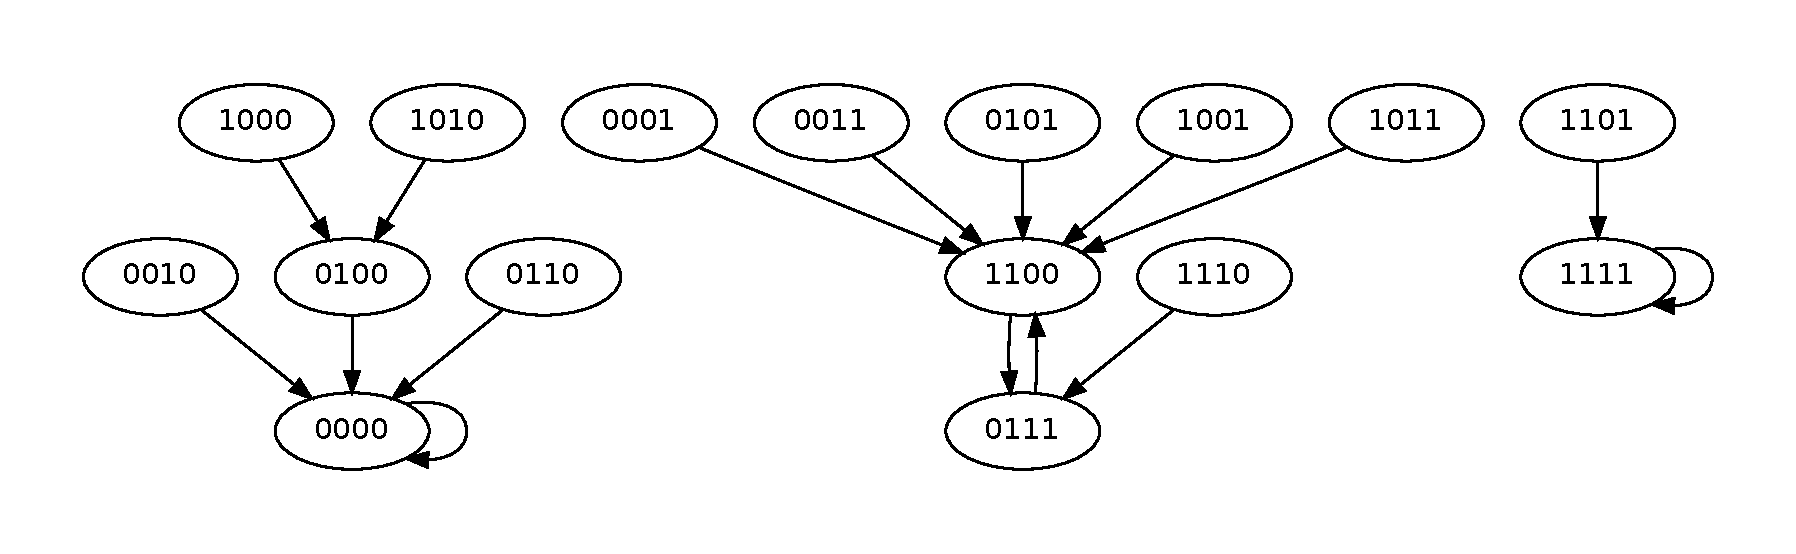
\includegraphics[scale=0.4]{./figuras/examp_2,1,1,2.pdf}
%\end{center}
%With this representation it is easy to visualize the attractors in the network dynamics as cycles in this graph (since $(\vec{x},\vec{y})$ is a transition in this graph if and only if $\vec{y}=F_S(\vec{x})$); thus, the loops in this graph, $(0,0,0,0)$ and $(1,1,1,1)$, are fixed points, and the cycle of length $2$ formed by state vectors $(1,1,0,0)$ and $(0,1,1,1)$ is a limit cycle with period length equal to $2$. 
%\end{exmp}

%\subsection{Gauss-Seidel Operator}

%In one of the first theoretical studies about update schedules in the context of automata networks \cite{robert}, F. Robert proved that Boolean networks without circuits have a unique fixed point. He also proposed a procedure, namely the Gauss-Seidel operator, which maps a network with asynchronous update (in our context, a sequential update schedule) into a synchronous model (ie, a parallel schedule). Specifically, for the sequential schedule $s(i)=i-1$, and a Boolean network $F$ of size $n$, the output of Gauss-Seidel operator is given by $F^{\prime}$, where the function $F^{\prime}(\cdot)=(f_1^{\prime}(\cdot),\cdots,f_n^{\prime}(\cdot))$ is defined as follows:
%\begin{align*}
%f_1^{\prime}(x) &= f_1(x)\\
%f_i^{\prime}(x)&=f_i(f_1^{\prime}(x),\cdots,f_{i-1}^{\prime}(x),x_i,\cdots,x_n),\quad \forall i=2,\cdots,n\\
%\end{align*}
%Robert proved that the iterative aplication of this operator on Boolean networks without circuits becomes stationary and the resulting network has the same fixed point than the original one (\cite{robert}). \par%The synchronous simulation of sequential update done by this operator has proven useful in itself in other fields (see for example, Chapter $6$ in \cite{trove.nla.gov.au/work/10029684}).\par
%Now, we define a transformation that receives a Boolean network, and outputs
Let $\mathcal{N}_n$ be the set of all Boolean networks of size $n$, and let $\mathcal{S}_n$ be the set of all block-sequential update schedules for Boolean networks of size $n$. We define the \textit{Gauss-Seidel} operator $\GS$ %:\mathcal{N}_n\times \mathcal{S}_n\rightarrow\mathcal{N}_n$, %which will be called as \textit{Gauss-Seidel operator}, 
as follows
\begin{align*} 
\GS:\mathcal{N}_n\times \mathcal{S}_n &\rightarrow\mathcal{N}_n\\
(F,s) &\mapsto F_s
\end{align*}
in this way, $\GS$ %Gauss-Seidel operator 
returns a network that simulates in parallel the dynamics of $F$ with scheme $s$. Since fixed points of Boolean networks are invariant under any block-sequential update, the network returned by $\GS$ %outputted by Gauss-Seidel operator 
exhibits the same fixed points of input network.%Or in other words
%$$\STG(F,S)=\STG(\GS(F,S),\pi)$$
%In one of the first theoretical studies about update schedules in the context of automata networks \cite{robert}, F. Robert proved that the iterative aplication of this operator, restricted to the sequential schedule $s(i)=i-1$, on Boolean networks without circuits becomes stationary and the resulting network has the same unique fixed point than the original one.

%that is, for a global transition function $F$ and a block-sequential update schedule $S$, $\GS(F,S)$ returns $F_S$, the global transition function of network $F$ with update schedule $S$, which complies that  
%$$\STG(F,S)=\STG(F_S,\pi)$$
%Last equality means that Gauss-Seidel operator returns the global transition function of a network that simulates in parallel the dynamics of $\STG(F,S)$, that is, one update of $F_S$ in parallel, produces the same output of one update of network $F$ with schedule $S$.

%\subsection{Filters}\label{subsec-filt}
%From the contribution of Robert of having applied the Gauss-Seidel operator in iterative manner, a line of investigation has initiated concerning the properties of this procedure. We need to introduce some notation necessary for the study and discussions conducted on this section and the rest of the entire work. 
For $(N,s) \in \mathcal{N}_n\times \mathcal{S}_n$ let $N^{i} = \GS(N^{i-1},S)$ be the network obtained after $i\geq 1$ applications of $\GS$. %Now, we are interested in applying iteratively the Gauss-Seidel operator.
%For a Boolean network $N$ and a block-sequential update schedule $S$, we define the \textit{Filter} associated to $N$ and $S$ as the following system
%\begin{align}
%\begin{split}\label{filt-def}
%N^0 &\equiv N \\
%N^{i+1} &\equiv \GS(N^i,S),\quad i\geq0
%\end{split}
%\end{align} 
%Clearly, s
Since the space of Boolean networks is finite and %Gauss-Seidel operator 
$\GS$ is deterministic, %after a finite number of steps %in the system (\ref{filt-def}),  
%Since the space of the Boolean networks of size $n$ is finite (there are $n$ local transition functions, and the number of possible non-equivalent Boolean functions of $n$ variables is bounded by the number of different truth tables of $n$ variables, then the total is at most $(2^{2^n})^n$), it ends up in a cycle of networks. Formally, 
it holds that there exist $t, p \in \mathbb{N}$ such that
%\begin{align}
%N^j &\neq N^{j+1},\quad j \in \{\bar{t},\ldots,\bar{t}+\bar{p}-1\}\\
$N^{t+ p} =N^{t}$. %\label{def-attr-net}
%\end{align}
We can take $t, p$ as the smallest integers that satisfy this equality. Thus, w%Analogously to the context of dynamical attractors of Boolean networks, %seen in Subsection \ref{subsec-attr}, we can talk here of 
%we refer to $\bar{t}$ and $\bar{p}$ as the \textit{transient} and the \textit{period} of network $N$, respectively. %as the smallest positive integers verifying this equality. %If there is no confusion about the initial network, we will refer to the transient and the period simply as $t$ and $p$. W
e define the \textit{filter attractor of network $N$ and scheme $s$, }$\mathcal{A}(N,s)$, as the set of Boolean networks of size $n$ which satisfy

$$\mathcal{A}(N,s)=\{N^{\ell} \quad| \quad \ell =t,\ldots,t+p-1\}$$ 

%We see that $|\mathcal{A}(N,S)|=p$; in the special case that $p=1$
When $\mathcal{A}(N,s)$ is a singleton, the filter attractor is said to be a \textit{structural fixed point}, while if $p>1$, the attractor is named a \textit{structural cycle}. It is clear that, since fixed points are preserved in each iteration of $\GS$, %in each iteration of (\ref{filt-def}), all networks produced in every iteration have the same fixed points, in particular those networks in the filter attractor.
all networks in $\mathcal{A}(N,s)$ share the same set of fixed points.
%Other interesting property shown by this procedure is the fact that, the parallel simulation of a network, in some manner reduces the comunication paths between nodes, which would result in a shortening of attractor periods, and finally a remotion or ``filtering'' of some limit cycles (if not all).

\begin{exmp}
Let $N$ be the disjunctive Boolean network of size $4$ given by the digraph below. Let $s$ be the block-sequential schedule with blocks $B_0=\{1,2\}$, $B_1=\{3,4\}$. After $2$ iterations of Gauss-Seidel operator, the filter converges to %the filter attractor, which is 
a structural cycle of period %length 
$2$. %formed by networks $N^2$ and $N^3=\GS(N^2,S)$.

\begin{tabular}{ccccccc}

\begin{minipage}{40 pt}
%\begin{figure}[h!]
%\captionsetup[figure]{labelformat=empty}
    \includegraphics[scale=0.6]{./figuras/ej_bueno.tex}
  %\centering
\textit{$N$}
%\end{figure}
\end{minipage}

&
\begin{minipage}{40 pt}
%\begin{figure}[h!]
%\captionsetup[figure]{labelformat=empty}
    \includegraphics[scale=0.7]{./figuras/arrow.tex}
  %\centering
%\end{figure}
\end{minipage}
&

\begin{minipage}{40 pt}
%\begin{figure}[h!]
%\captionsetup[figure]{labelformat=empty}
    \includegraphics[scale=0.6]{./figuras/ej_bueno_1.tex}
  %\centering
\textit{$N^1$}
%\end{figure}
\end{minipage}

&
\begin{minipage}{40 pt}
%\begin{figure}[h!]
%\captionsetup[figure]{labelformat=empty}
    \includegraphics[scale=0.7]{./figuras/arrow.tex}
  %\centering
%\end{figure}
\end{minipage}
&

\begin{minipage}{40 pt}
%\begin{figure}[h!]
%\captionsetup[figure]{labelformat=empty}
    \includegraphics[scale=0.6]{./figuras/ej_bueno_2.tex}
  %\centering
\textit{$N^2$}
%\end{figure}
\end{minipage}

&
\begin{minipage}{40 pt}
%\begin{figure}[h!]
%\captionsetup[figure]{labelformat=empty}
    \includegraphics[scale=0.7]{./figuras/arrows.tex}
  %\centering
%\end{figure}
\end{minipage}
&


\begin{minipage}{40 pt}
%\begin{figure}[h!]
%\captionsetup[figure]{labelformat=empty}
    \includegraphics[scale=0.6]{./figuras/ej_bueno_3.tex}
  %\centering
\textit{$N^3$}
%\end{figure}
\end{minipage}

\end{tabular}


Below there are the state transition digraphs of $N$, $N^2$ and $N^3$ under parallel dynamics. We can see that network $N$ has $3$ attractors: $2$ fixed points, and $1$ limit cycle of length $2$. In the other hand, $N^3$ only has $2$ fixed points, while $N^2$ has the same attractors as $N$. All networks have the same fixed points.

\begin{multicols}{2}
\begin{center}
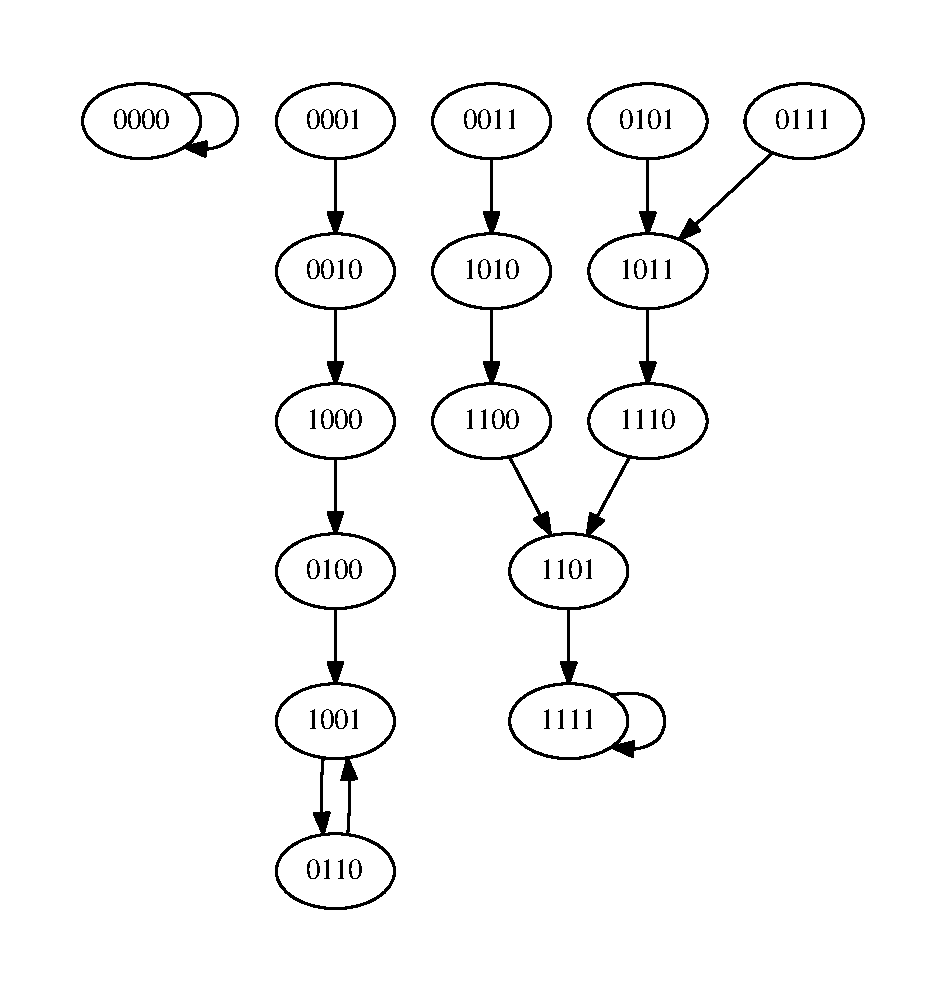
\includegraphics[scale=0.3]{./figuras/ej_bueno_1,1,1,1.pdf}
\textit{$\STG(N,\pi)$}
\end{center}
\begin{center}
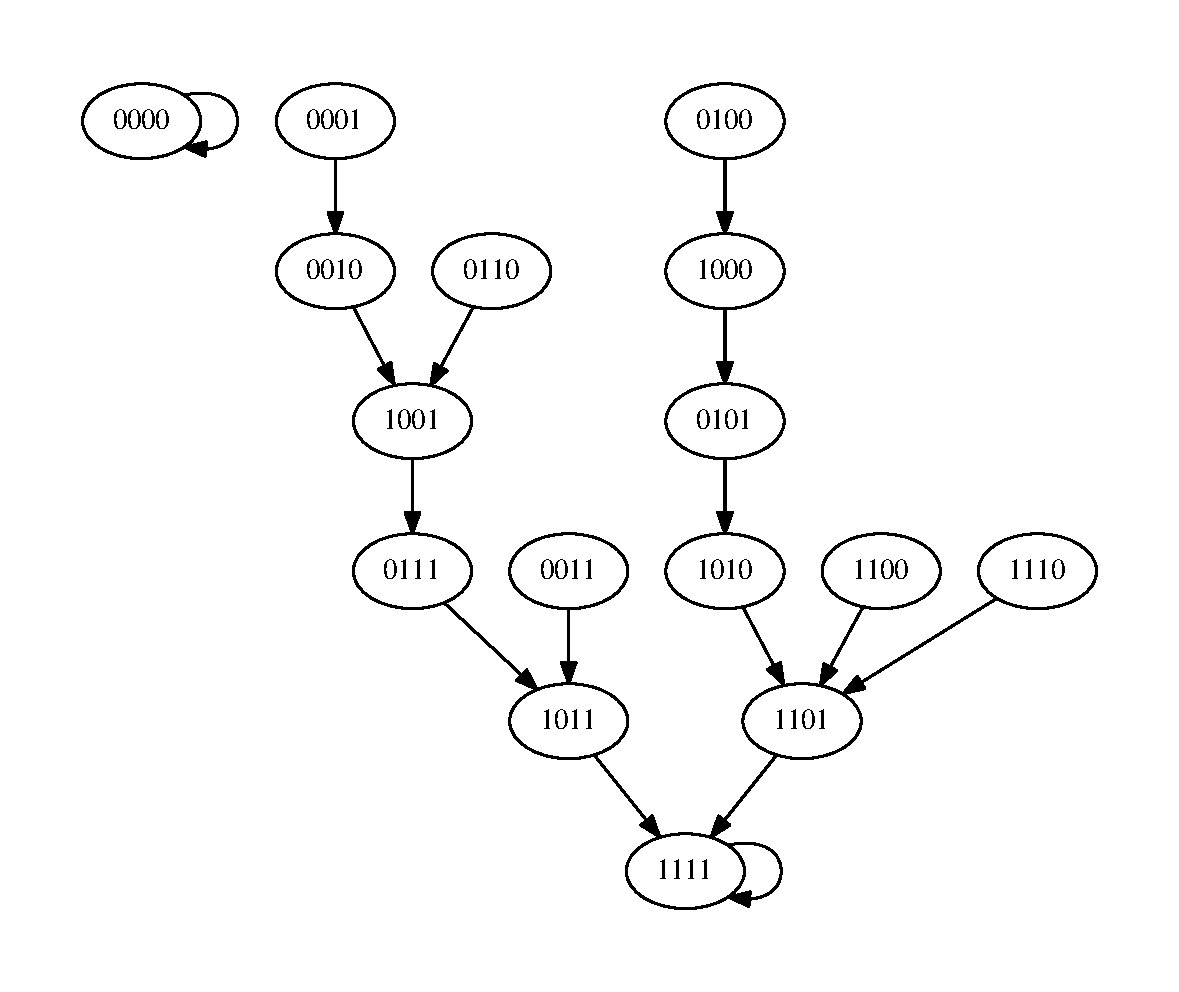
\includegraphics[scale=0.3]{./figuras/3_1,1,2,2_ej_bueno_1,1,1,1.pdf}
\textit{$\STG(N^3,\pi)$}
\end{center}
\end{multicols}
\begin{center}
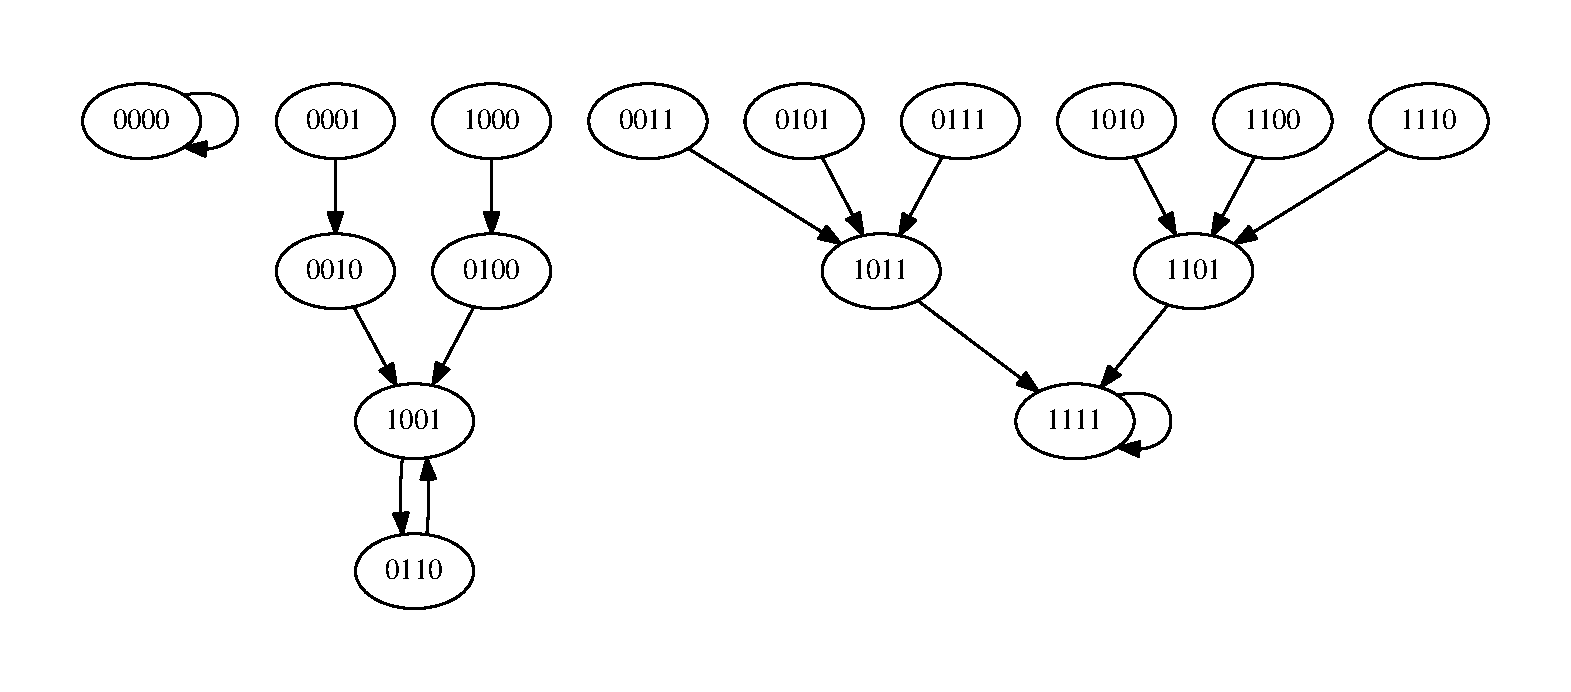
\includegraphics[scale=0.3]{./figuras/4_1,1,2,2_ej_bueno_1,1,1,1.pdf}
\textit{$\STG(N^2,\pi)$}
\end{center}
\end{exmp} 

\section{Convergence complexity}\label{sec-filt-conv}

\subsection{Size of the transient}       

The main result of this section is the following theorem  

\begin{teo}\label{teo-conv-gen}
Let $D=(V,A)$ be a disjunctive Boolean network, and a block-sequential update schedule $s$ for this network. Then, in $\mathcal{O}(|V|^2)$ executions of $\proc{Gauss-Seidel}$, the filter converges to an attractor.
\end{teo}

To prove this theorem, we will restrict first to the case of schedules with only \textbf{two} blocks. For a Boolean network $F$ with digraph $D=(V,A)$, and some update scheme $s$, we will refer to the digraph of network $F_s$ returned by $\GS(F,s)$ as $D^s=(V,A^s)$. To model this situation, it is proposed the following: given the subdigraph of the network induced by the nodes in $B_0$, %which we assume it has $q$ nodes ($|B_0|=q$), 
and some arbitrary fixed node $a \in B_1$, we define the state vector $\vec{x}(a,D) \in \{0,1\}^{|B_0|}$ representing, for each node $i$ in $B_0$, if there exists an arc starting from $i$ and ending on $a$:  

\begin{equation}\label{def-vect-filt}
\forall i \in \{1,\ldots,|B_0|\},\quad x(a,D)_i=1\quad \Longleftrightarrow\quad (i,a) \in A \quad (s(i)<s(a))
\end{equation}

If $(u,v)$ is an interior arc of the first block ($u,v \in B_0$), and $x(a,D)_v=1$, after applying the algorithm the output network $D^s$ satisfies $x(a,D^s)_u=1$. It is enough to have a single arc $(u,v)$ of all those that depart from $u$ verifying the above, to have that $x(a,D^s)_u=1$. This is similar to what happens with a disjunctive Boolean network, % where the transition local functions are $OR$ functions (disjunctions of variables)
%: here 
where it is enough that some parent of node $u$ has state equal to $1$, to have that the state of $u$ equals $1$ in the next iteration. If we consider a Boolean network $D(B_0)^T=(B_0,E^T)$, where $E^T$ is the set of arcs that results from reversing the arcs of $D(B_0)$%(the adjacency matrix of $D(B_0)^T$ is the transpose of the adjacency matrix of $D(B_0)$)
, with local transition functions given by $OR$ functions, we could simulate the effect of applying $\proc{Gauss-Seidel}$ on $D$ and $s$. More precisely, let $M \in \mathcal{M}_{|B_0|\times |B_0|}(\{0,1\})$ be the adjacency matrix of $D(B_0)^T$, the subdigraph induced in $D$ by $B_0$ with reversed arcs, that is,  
$M_{ij}=1$ if and only if $(j,i)\in A$, where $i,j \in B_0$. Then, the following holds.

\begin{lema}\label{l2}
Let $D=(V,A)$ be a disjunctive network, and a block-sequential update schedule $S$ for this network, with only two blocks $B_0$ and $B_1$. Let $a \in B_1$ be a node in the second block. 
Then $\vec{x}(a,D^S) =\vec{x}(a,D)\cdot M$.
\end{lema}

As a consequence of previous lemma, iterated applications of $\proc{Gauss-Seidel}$ algorithm on an input network can be simulated by integer powers of the adjacency matrix. This allows to prove the restriction of the main theorem for two blocks.

\begin{prop}\label{l6}
Let $D=(V,A)$ be a disjunctive Boolean network, and a block-sequential update schedule $s$ for this network which has only two update instants or blocks $B_0$ and $B_1$. Then, in $\mathcal{O}(|B_0|^2)$ executions of $\proc{Gauss-Seidel}$, the filter converges to an attractor.
\end{prop}

\begin{proof}[Proof of Proposition \ref{l6}]
Let $s$ be the update function of $S$. First suppose that $D$ has no arcs $(u,v)$ where $u \in B_0$ and $v \in B_1$. Since $s(u)\geq s(v)$ for every arc $(u,v)$ in $D$, $\proc{Gauss-Seidel}$ adds to $D^S$ every arc of $D$ without changes and then returns (Note \ref{pseudocode}, \ref{subsec-comp-gs}). Therefore $D$ is a structural fixed point reached after one execution of $\proc{Gauss-Seidel}$.\par

Assume now that there is an arc $(i,a) \in A$ such that $s(i)<s(a)$, meaning that the vector $\vec{x}(a,D)$ is not null. Let $M \in \mathcal{M}_{|B_0|\times |B_0|}(\{0,1\})$ be the adjacency matrix of the subdigraph induced in $D$ by the first block, $D(B_0)$, with inverted arcs, ie:
$$M_{ij}=1 \Longleftrightarrow (j,i)\in A, j,i \in B_0$$
Then, by the Lemma \ref{l2}, for every $n \in \mathbb{N}$, $\vec{x}(a,D^n) =\vec{x}(a,D)\cdot M^n$, where $D^n$ is the digraph obtained after $n$ iterated executions of $\proc{Gauss-Seidel}$ over $D$ (with schedule $S$). Thus, we see the iterated application of $\proc{Gauss-Seidel}$ is equivalent (Note \ref{rel-mat-net}) to the parallel update of network $D(B_0)^T$, the subdigraph induced in $D$ by the first block with transposed arcs, with initial condition $\vec{x}(a,D)$. By Note \ref{mainteo}, there exist $t \in \mathcal{O}(|B_0|^2)$, $p \in \mathbb{N}$, such that 
\begin{equation}\label{eq-gen-case-2}
\vec{x}(a,D^{t+p})=\vec{x}(a,D^{t}) 
\end{equation}

%Arcs connecting nodes in the same block are always preserved by $\proc{Gauss-Seidel}$. 
Assume that there is an arc $(j,k) \in A$ such that $s(j)>s(k)$ -this arc $(j,k)$ is preserved without changes by $\proc{Gauss-Seidel}$ (Note \ref{pseudocode})-, an arc $(i,a) \in A$ such that $s(i)<s(a)$, and a directed path in $D(B_0)$ from $k$ to $i$ of length $p \in \mathcal{O}(|B_0|)$, or equivalently, $M_{i,k}^p>0$. Given that $x(a,D)_i > 0$, from Lemma \ref{l2} it follows that $x(a,D^p)_k > 0$, namely there is in $D^p$ an arc $(k,a)$, where $s(k)<s(a)$. By Lemma \ref{caract_disj}, %the definition of $\proc{Gauss-Seidel}$ algorithm, 
in $D^{p+1}$ is added the arc $(j,a)$, where $j, a$
%$s(j)=s(a)=1$, meaning that $\proc{Gauss-Seidel}$ is adding an arc that connects nodes 
belong to the second block $B_1$. These arcs are not described by the vectors $\vec{x}(a,D)$ %(because the components of these vectors depict nodes in the first block) 
and are added after 
%in the iteration $p+1 \in 
$\mathcal{O}(|B_0|)$ iterations of $\proc{Gauss-Seidel}$. \par%These arcs remain in the digraphs $D^m$, with $m\geq p+1$.\par
The foregoing paragraph and equality (\ref{eq-gen-case-2}) show that in at most $\mathcal{O}(|B_0|^2)$ executions of $\proc{Gauss-Seidel}$ over $D$ with schedule $S$, this iterative procedure outputs a network in the filter attractor $\mathcal{A}(D,S)$.\par
\end{proof}

\begin{exmp}
In the images below there is a disjunctive network $D$ of seven nodes, and a block-sequential update schedule of two blocks for this network, where nodes in the first block $B_0$ are orange, and in the second block are blue. We see the subdigraph induced by the first block, $D(B_0)$, is strongly connected and primitive: it has a circuit of length $5$ and other of length $4$. Moreover it is known that for the adjacency matrix $M$ of $D(B_0)$ of this example, only after $17=(5-1)^2+1=(|B_0|-1)^2+1 \in \mathcal{O}(|B_0|^2)$ applications of $\proc{Gauss-Seidel}$ onto network $D$, the filter attractor -a structural fixed point- is reached (see the definition and general bounds for the exponent of a primitive matrix \cite{mat_book}). Observe that the arc $(6,7)$ appears in the third application of $\proc{Gauss-Seidel}$: these arcs appear after a number of iterations linear on $|B_0|=5$.

\begin{multicols}{2}
\begin{center}
\includegraphics[scale=0.4]{./figuras/ejpr.tex}
$$D$$
\end{center}
\begin{center}
\includegraphics[scale=0.4]{./figuras/ejpr_1.tex}
$$D^{17}$$
\end{center}
\end{multicols}
\end{exmp}

We are able now to prove the main theorem, using last result.

\begin{proof}[Proof of Theorem \ref{teo-conv-gen}]
The case remaining to prove is when the schedule $s$ has more than $2$ update blocks $(B_{\ell})_{\ell \in L, |L|>2}$. Assume there is an arc $(i,j) \in A$ such that $s(i)=\ell_i<s(j)=\ell_j$ (otherwise none arc is changed, by Note \ref{pseudocode}, \ref{subsec-comp-gs}, and the current network is a filter attractor). The evolution of the arcs originated by $(i,j)$ through iterative applications of $\proc{Gauss-Seidel}$ depends on the topology of subdigraph $D_{\ell_j}\equiv D(B_0\cup\ldots\cup B_{\ell_j -1})$, because once it is produced an arc $(v_i,j)$ where $s(v_i)\geq s(j)$, this arc is preserved without changes in ulterior iterations.\par
In at most $|D_{\ell_j}| \in \mathcal{O}(|V|)$ iterations of $\proc{Gauss-Seidel}$, the arcs originated by $(i,j)$ reach all the non-trivial s.c.c. reachable in $D_{\ell_j}$. Any non-trivial s.c.c. $C$ of $D_{\ell_j}$ could belong to one or more than one block. In the first case, $C$ is preserved without changes after applying $\proc{Gauss-Seidel}$ (no new arcs are added since this would imply the existence of circuits of $C$ belonging to different blocks). Since $C$ is preserved and $\proc{Gauss-Seidel}$ is deterministic, the evolution of arcs starting from it and ending on $j$, is equivalent to the dynamics of the filter applied on the network $D(C)\cup \{j\}$ with the schedule of two blocks $B_0^{\prime}=V(D(C))$ and $B_1^{\prime}=\{j\}$. Then, by Proposition \ref{l6}, after $\mathcal{O}(|D(C)|^2)\subseteq\mathcal{O}(|V|^2)$ executions of $\proc{Gauss-Seidel}$, the initial filter restricted to $D(C)$ (and the arcs ending on $j$) converges to an attractor.\par
Suppose now there is a non-trivial s.c.c. $C$ of $D_{\ell_j}$ belonging to more than one block, which receives at some iteration an arc ending on $j$. This s.c.c. has necessarily some arcs which will be changed by executions of $\proc{Gauss-Seidel}$. $C$ produces after every $\proc{Gauss-Seidel}$ iteration a subdigraph $C^m$ in $D_{\ell_j}^m, m\geq 0$, which by Lemma \ref{cfc} has exactly one non-trivial s.c.c. in $D_{\ell_j}^m$. This subdigraph $C^m$ has some fixed subdigraphs $C^m(B_{\ell})$ induced by the different blocks in which $C$ (or $C^m$) is contained, plus maybe some additional arcs added after $\mathcal{O}(|V|)$ iterations. Even if there are arcs of $C^m$ which connect different blocks that are changing after every iteration, the number of iterations required to propagate arcs ending on $j$ to these subdigraphs $C^m(B_{\ell})$ is $\mathcal{O}(|V|)$. Once this has happened, by the same argument in previous paragraph, after $\mathcal{O}(|C^m(B_{\ell})|^2)\subseteq\mathcal{O}(|D(C)|^2)\subseteq\mathcal{O}(|V|^2)$ executions of $\proc{Gauss-Seidel}$, the initial filter restricted to $C^m(B_{\ell})$ (and the arcs ending on $j$) converges to an attractor.  
\end{proof}

\subsection{Size of the attractor}

Last subsection showed that the transient length of filters applied to disjunctive networks can be bounded polynomially on the size of the network. Unfortunately, this statement does not apply for the period length: it happens that limit cycles of different lengths produced by distinct strongly connected components, interact with each other by multiplying its lengths, which quickly increases the size of the filter attractor. Next theorem shows this effect in networks having disconnected cycles with different lengths, but it is easy to produce this same effect even with cycles with different lengths belonging to the same weakly connected component of the network.

\begin{teo}\label{teo-superpol}
There is a family of disjunctive Boolean networks $(D_n)_{n \geq 3}$, and a family of block-sequential update schedules $(S_n)_{n \geq 3}$ of two blocks, such that, the filter applied to $(D_n,S_n)$, for every $n \in \mathbb{N}, n \geq 3$ exhibits super polynomial period length.  
\end{teo}

\begin{proof}
Let $n$ be a positive integer, $\pi(n)$ be the number of primes not exceeding $n$, and $\{p_1,p_2,\ldots,p_{\pi(n)}\}$ be the first $\pi(n)$ primes. The network $D_n=(V_n,A_n)$ has a set of $|V_n|=1+\sum_{i=1}^{\pi(n)} p_i$ vertices arranged as follows: there are $\pi(n)$ cycles, each one of length $p_i$ and connected through an arc starting on the cycle and ending on a common single vertex $v_c$ as the figure shows. The schedule $S_n$ has two blocks, where the first block to be updated has cyan nodes, and the second block has one orange node (the node $v_c$).
\begin{center}
\includegraphics[scale=0.8]{./figuras/cyc_prim.tex}
\end{center}
If we iterate Gauss-Seidel over network $D_n$ and schedule $S_n$, the procedure does not loop by producing some network produced before since the networks produced are all different. We only recover the initial network after $lcm\{p_1,p_2,\ldots,p_{\pi(n)}\}=\prod_{i=1}^{\pi(n)} p_i$ applications of Gauss-Seidel. Or in other words, if we refer to the network obtained after $k\geq 0$ applications of Gauss-Seidel on $(D_n,S_n)$ as $D_n^k$, it holds that
\begin{equation}\label{evol-loop}
D_n^{lcm\{p_1,p_2,\ldots,p_{\pi(n)}\}}=D_n^0=D_n, \quad\forall n\geq 3
\end{equation}
therefore, the transient length is $0$ and the period length is equal to $lcm\{p_1,p_2,\ldots,p_{\pi(n)}\}$.
To obtain a lower bound of the period length, we follow the argument of Montealegre \& Goles (2014) \cite{monteal} and Kiwi et al (1994) \cite{Kiwi1994527} to state that the period length is superpolynomial, that is, it is lower bounded by $\exp(\Omega(\sqrt{|V_n|\cdot \log|V_n|}))$ and is not bounded by any polynomial in $|V_n|$.
\end{proof}


\section{Filtering dynamic cycles}\label{sec-filt-cyc}

In this section we will see a strategy to remove the dynamic cycles from networks in the filter attractor. For that purpose, we need the following definitions. 

\begin{defn}[Induced length]\label{del-il}
Let $C\subseteq D=(V,A)$ be a cycle (or a simple directed circuit), and let $s$ be a block-sequential update schedule for network $D$ with $m\geq 1$ blocks $(B_j)_{j=0}^{m-1}$. Let $0\leq i_C \leq m-1$ be the instant such that $B_{i_C}$ is the last block of those induced by $s$ having nodes from the circuit $C$. The \textit{induced length of }$C$\textit{ with respect to }$s$, denoted by $\mathcal{IL}(C,s)$, correspond to the quantity of nodes of $C$, that belong to block $B_{i_C}$.
\end{defn}

\begin{exmp}
In the image below at left there is a disjunctive network $D$ of nine nodes, and a block-sequential update schedule $s$ of three blocks for this network, where nodes in the first block $B_0$ are green (nodes $8,4,5$), nodes in the second block $B_1$ are blue (nodes $9,6$) and those in the third block $B_2$ are orange (nodes $1,2,3,7$). In the table below at right we can see several cycles of $D$, each of them with its respective last block and induced length:

\begin{multicols}{2}
%\begin{center}
\includegraphics[scale=0.6]{./figuras/ejil.tex}
$$D$$
%\end{center}
\begin{center}
\begin{tabular}{c|c|c}
\hline
\textbf{Cycle }$C$ &  \textbf{Instant } $i_C$ & $\mathcal{IL}(C,s)$\\
\hline
  $(1,2,3,4,5,9)$ & 2 & 3 \\
  $(1,2,3,4,5,8,9)$ & 2 & 3 \\
  $(5,6,7,8)$ & 2 & 1 \\
  $(1,2,3,4,5,6,7,8,9)$ & 2 & 4 \\
  $(8,5)$ & 0 & 2 \\
\end{tabular}
\end{center} 
\end{multicols}

Notice that the case of circuit $(8,5)$ is the same of all those circuits connecting nodes pertaining to the same block. Here the induced length of the circuit is equal to the usual cycle length.
\end{exmp}

We can now state a condition on the input network and schedule that ensures networks in the filter attractor do not have limit cycles. We will refer to this condition as \textit{cycle-filter}.

\begin{defn}[Cycle-filter condition]\label{cond}
Let $D=(V,A)$ be a disjunctive Boolean network, and consider a block-sequential update schedule $s$ for this network. The pair $(D,s)$ is \textbf{cycle-filter} if every non-trivial strongly connected component of digraph $D$\\
(i)  Contained in just one updating block induced by schedule $S$ is primitive.\\
(ii) Belonging to more than one updating block induced by schedule $S$, verifies that the greatest common divisor of the induced lengths of its simple circuits equals $1$. 
\end{defn}

We have now the elements to enunciate the main result of this section.

\begin{teo}\label{filt}
Let $D=(V,A)$ be a disjunctive Boolean network, and $S$ a block-sequential update schedule for this network. If $(D,S)$ is cycle-filter, then the networks in $\mathcal{A}(D,S)$ do not have limit cycles when updated with the parallel schedule $\pi$. 
\end{teo}

The manner in which the limit cycles are removed, is by means of the following equivalence
\begin{center}
\textit{Parallel dynamics of a digraph $D$ does not have limit cycles if and only if each s.c.c. of $D$ is primitive}
\end{center}
which is a consequence of a known fact relating the structure with the parallel update of a digraph (see Lemma 6 \cite{disj}). Thus, our aproach to filter limit cycles is to ensure that every strongly connected component of networks in the filter attractor is primitive. We need now a relation between the structure of input network, and the networks in its filter attractor. The following proposition will be useful in that direction, which in turn shows the utility of the induced length of a cycle.

\begin{prop}\label{ind_l}
Let $D=(V,A)$ be a disjunctive Boolean network, and a block-sequential update schedule $s$ for this network with $m\geq 1$ blocks $(B_j)_{j=0}^{m-1}$. If there is a simple circuit $C$ in $D$, such that $\mathcal{IL}(C,s)=L$, then there is a circuit of length equal to $L$ in every network in $\mathcal{A}(D,s)$.
\end{prop} 

With this proposition, the main result can be proved.

\begin{proof}[Proof of Theorem \ref{filt}]
Let $(D,s)$ be a pair digraph-schedule which is cycle-filter and let $\bar{D}$ be a network in $\mathcal{A}(D,s)$, the filter attractor of the pair $(D,s)$. By applying inductively Lemma \ref{cfc}, every non-trivial s.c.c. $C$ of $D$ produces at most one non-trivial s.c.c. $\bar{C}$ in $\bar{D}$. Whenever a non-trivial s.c.c. $C$ of $D$ is studied in isolation from the rest of the digraph, %the Lemma \ref{varios} is being used implicitly, that is, if $C$ belongs to the first $n$ blocks of $S$, we use the schedule $S^{\prime}$ resulting in restricting $S$ to its first $n$ blocks and the subdigraph $D(C)$ of $D$ induced by the nodes of $C$. T
the conclusions drawn for $D(C)$ are also valid for $D$ thanks to Lemma \ref{varios}.\par
Let $C$ be a non-trivial strongly connected component in $D$, and suppose first $C$ is completely contained in just one block induced by $s$, implying $C$ is preserved in every application of $\proc{Gauss-Seidel}$, and thus, $C$ is a s.c.c. in $\bar{D}$. It holds that %We first show by contradiction that 
no new circuits are added to $C$. %On the contrary, i
If this were the case, the Lemma \ref{caract_disj} says that a circuit $\bar{C}$ in $C$ appearing in any of the applications of $\proc{Gauss-Seidel}$ is equivalent to the existence of a circuit $C^*$ in $D$ connecting the nodes connected by $\bar{C}$ and some other nodes that are not in the block of $C$ (as $\bar{C}$ was not originally in $C$). This means that $C$ belongs to more than one block, which is absurd. Since $(D,s)$ is cycle-filter, $C$ is primitive, and in this way, it holds that every s.c.c. of $D$ contained in just one updating block ends up in $\bar{D} \in \mathcal{A}(D,s)$ as a primitive s.c.c.\par
Now let $C$ be a non-trivial s.c.c. of $D$ belonging to more than one block. If $C$ consists of only one simple circuit $\mathcal{C}$, as $(D,s)$ is cycle-filter then $\mathcal{C}$ has induced length with respect to $s$ equal to $1$. Then by Proposition \ref{ind_l}, the s.c.c. $\bar{C} \in \bar{D}$ generated by $C \in D$ has a loop and therefore $\bar{C}$ is primitive. If $C$ is comprised of several circuits, since $(D,s)$ is cycle-filter the greatest common divisor of its induced lengths is $1$, or in other words, the set of induced lengths of cycles in $C$ is setwise coprime. By Proposition \ref{ind_l}, the s.c.c. $\bar{C} \in \bar{D}$ generated by $C \in D$, has a circuit of length $L$ for every circuit in $C$ of induced length $L$. Therefore, the set of lengths of cycles in $\bar{C}$ is also setwise coprime, implying that %$k(\bar{D}(\bar{C}))=1$ and 
$\bar{C}$ is primitive. %This shows that, if $(D,S)$ is cycle-filter, every non-trivial s.c.c. $\bar{C}$ of any network $\bar{D}$ in $\mathcal{A}(D,S)$ is primitive, which implies by Lemma \ref{primcyc} (employing the parallel schedule $\pi$ in the hypothesis of the lemma) that the state of every s.c.c. $\bar{C}$ of $\bar{D}$ is fixed in all attractors of $\STG(\bar{D},\pi)$, meaning that the dynamic of $\STG(\bar{D},\pi)$ does not have limit cycles. This shows the condition sufficiency.    
\end{proof}


\appendix

\section{Proofs}\label{sec-proof}

\subsection{Characterization of Gauss-Seidel network}

In this subsection it is presented one of the fundamental tools employed in this work, given by the framework of disjunctive networks. Recall that for a Boolean network $F$ with digraph $D=(V,A)$, and some update scheme $S$, we will refer to the digraph of network $F_S$ returned by $\GS(F,S)$ as $D^S=(V,A^S)$. %For a network $D=(V,A)$ with global transition function $F$, and some update schedule $S$, it was already noticed in Section \ref{defini} that the network returned by Gauss-Seidel operator, which we name as $D^S=(V,A^S)$, is the network whose global transition function corresponds to $F_S$. 
If the component function of $F_S$ associated to node $i \in V$ is $f_i^S$, then the set of arcs $A^S$ of the network $D^S$ corresponds %(since it is the digraph associated to the network with global transition function $F_S$) 
to the following:

$$A^S=\{(j,i) |\quad f_i^S(\vec{x}) \text{ depends on } x_j\}$$ 

The following lemma is a characterization of this set $A^S$, that will be very useful for subsequent arguments, since it relates the arcs of network $D^S$ to arcs from the input network $D$. The proof of this result can be reviewed on \cite{disj}. %and it is exposed here by the importance of this characterization throughout this entire work.
    
\begin{lema}[\cite{disj}]\label{caract_disj}
Let $D=(V,A)$ be a Boolean disjunctive network, and let $S$ be a block-sequential update schedule, with update function $s$. The set of arcs $A^S$ of the network $D^S$ returned by Gauss-Seidel on $(D,S)$ is characterised by 
\begin{align*}
A^S &= \{(j,i)| \text{ there exists in $D$ a path } (v_0,v_1,\ldots,v_l) \text{ from } j=v_0\\
&\qquad\text{ to } i=v_l\text{ such that } s(v_0)\geq s(v_1) \wedge \forall 1\leq k < l, s(v_{k})<s(v_{k+1}) \}
\end{align*}
\end{lema}

\subsection{Computing the Gauss-Seidel operator}\label{subsec-comp-gs}
\begin{note}\label{pseudocode}
It is possible to write an algorithm that returns the network $D^S=(V,A^S)$ calculated by the Gauss-Seidel operator associated to a certain block-sequential update schedule $S$ applied onto an input disjunctive network $D=(V,A)$. Essentially, this algorithm visits every block of the schedule according to their order, and passes over each incident arc $(u,j)$ to some node $j$ in the block, executing different actions depending on the update times. Whether $s(u)\geq s(j)$, the arc $(u,j)$ is added to the set $A^S$ without changes. Otherwise, an arc $(t,j)$ is added to $A^S$ for every arc $(t,u) \in A^S$. The correctness proof of this algorithm as well as its time complexity can be revised in \cite{mitesis}.
\end{note}

%The following pseudo-code is the formalization of the algorithm that returns the network $D^S=(V,A^S)$ calculated by the Gauss-Seidel operator associated to a certain block-sequential update schedule $S$ (received as input) applied onto an input network represented as a digraph $D=(V,A)$. Thus, the following algorithm provides a procedural characterization of Gauss-Seidel operator.      
%\begin{codebox}
%\Procname{$\proc{Gauss-Seidel}(D=(V,A),S)$}
%\li $A^{\prime} \gets \phi,\quad (A^{\prime}\subseteq A)$\>\>\>\>\quad\Comment initialization 
%\li $I \gets \phi,\quad (I\subseteq V)$
%\zi \text{Let $B_0,\ldots,B_{m-1}$ be the blocks of $S$, and let $s$ be the update function}
%\li \For $i \gets 0$ \To $m-1$
%\li  \Do \For $j \in B_i$ 
%\li \Do \For $ (u,j) \in A$ \>\>\>\>\quad\Comment we go over every arc incident to node $j$ \label{3rd-for}
%\li \Do \If $s(u)\geq s(j)$
%\li \Do $A^{\prime} \gets A^{\prime} \cup \{(u,j)\}$ \label{linea7}
%\li  \ElseNoIf
%\li \For $(t,u)  \in A^{\prime}$
%\li  \Do$A^{\prime} \gets A^{\prime} \cup \{(t,j)\}$\label{second_act} 
%\End
%\End
%\End
%\li 
% $I\gets I\cup \{j\}$
%\End
%\End
%\li \Return $(I,A^{\prime})$
%\end{codebox}
%The correctness proof of $\proc{Gauss-Seidel}$ algorithm can be revised in Lemma A.3 \cite{mitesis}. It is not difficult to see from this algorithm that Gauss-Seidel operator, when applied onto a disjunctive Boolean network $(V,A)$ of size $n=|V|$ and a block-sequential update schedule, can be computed on time at most $\mathcal{O}(|V|\cdot|A|)=\mathcal{O}(n^3)$ (Proposition 4.1 \cite{mitesis}).  


\subsection{Proofs for Section \ref{sec-filt-conv}}


\begin{proof}[{Proof of Lemma \ref{l2}}]
Let $s$ be the update function of schedule $S$. Suppose it is not true, that there exists $i \in B_0$ such that $(\vec{x}(a,D)\cdot M )_i=1$ and $x(a,D^S)_i=0$. Assume the arcs in $A$ whose starting node is $i$ are the following:

$$\{(i,j)\}_{j \in H}, \quad H \subseteq V$$

Since $(\vec{x}(a,D)\cdot M)_i=1$, necessarily there exists $j \in H \cap B_0$ satisfying $x(a,D)_j=1$. If it was that for all $k$ in $H \cap B_0$, $x(a,D)_k=0$, it would hold that 

\begin{align*}
(\vec{x}(a,D)\cdot M)_i &=\sum_{k \in B_0} x(a,D)_k M_{ki}\\  
&= \sum_{k \in B_0 \cap H} \underbrace{x(a,D)_k}_{=0} M_{ki} + \sum_{k \in B_0/H} x(a,D)_k \underbrace{M_{ki}}_{=0} = 0
\end{align*}

which would be absurd. Since there exists $j \in H \cap B_0$ satisfying $x(a,D)_j=1$, from definition of $\vec{x}(a,D)$, we know $(j,a) \in A$ with $s(j)<s(a)$. From Lemma \ref{caract_disj}, it holds that $(i,a)$ is an arc of digraph $D^S$, or in other words,
%Observe since $j \in H$, this means $(i,j) \in A$. When $\proc{Gauss-Seidel}$ is applied over $D$ and $S$, the first block processed is $B_0$, implying the arc $(i,j)$ is processed (when node $j$ is processed) before the arc $(j,a)$ (which is processed when node $a$ is processed). From what was said before: $s(i)=s(j)<s(a)$, then $(i,j)$ is processed at line \ref{linea7} from $\proc{Gauss-Seidel}$, and $(j,a)$ is processed at line \ref{second_act}: thus, the arc $(i,j)$ is added to $A^{\prime}$, and since $(i,j) \in A^{\prime}$ when $(j,a)$ is processed, then the arc $(i,a)$ is added to $A^{\prime}$. With this, 
 $x(a,D^S)_i=1$, which contradicts the initial assumption.\par

Suppose now there exists $i \in B_0$ such that $(\vec{x}(a,D)\cdot M)_i=0$ and $x(a,D^S)_i=1$, or in other words, $(i,a)$ is an arc of digraph $D^S$. %Since $x(a,D^S)_i=1$, it holds (see \ref{subsec-comp-gs}) that $(i,a) \in A^{\prime} (s(i)<s(a))$. At this point w
We can use the Lemma \ref{caract_disj} again to state that there is in $D$ a path $(v_0,v_1,\ldots,v_{\ell})$ from $i=v_0$ to $a=v_{\ell}$ such that: 
\begin{align}
s(v_0)\geq & s(v_1) \label{A1} \\
\forall 1\leq k < \ell, s(v_{k}) <& s(v_{k+1}) \label{A2}
\end{align}  

Since there are only two blocks, from (\ref{A1}) we see $v_1 \in B_0$ (and therefore, it is different from $a$), and from (\ref{A2}), it is deduced $\ell=2$. With this we have $(i,v_1) \in A$, meaning that $M_{v_1,i}=1$. Now, since $(v_1,a) \in A$ y $s(v_1) < s(a)$, this allows to say that $x(a,D)_{v_1}=1$. Considering the foregoing:

$$(\vec{x}(a,D)\cdot M)_i=\sum_{k \in B_0} x(a,D)_k M_{ki} \geq x(a,D)_{v_1} M_{v_1,i}=1$$

which is absurd.

\end{proof}

The proof of the next lemma can be reviewed on \cite{disj}.
\begin{lema}[\cite{disj}]\label{cfc}
Let $D$ be a strongly connected digraph and $s$ a block-sequential update schedule of its nodes. Then, $D^s=\proc{Gauss-Seidel}(D,s)$ is comprised of one unique non-trivial strongly connected component and possibly some outgoing acyclic subdigraphs. 
\end{lema}

\subsection{Proofs for Section \ref{sec-filt-cyc}}

\begin{proof}[Proof of Proposition \ref{ind_l}]
Assume first the simple circuit $C$ of $D$ is contained in only one block. This circuit is preserved after every iteration of $\proc{Gauss-Seidel}$ (Note \ref{pseudocode}, \ref{subsec-comp-gs}), and the statement holds trivially. Assume now that $C$ is contained in more than one block. Without loss of generality, consider one directed path $P=(o,v_1,\cdots,v_i,v_{i+1},\cdots v_{l-1},e)$ formed by a directed sequence of arcs from $C$, such that for every node $a \in V$ connected by $P$ with $a\neq o,e$, $s(a)<s(o)=s(e)$, and $o,e$ belong to the last block where $C$ has nodes. We will say this is the $i_C-$th block. We observe that in $P$, there are arcs $(m,n)$ verifying either $s(m)\geq s(n)$ or $s(m) < s(n)$. In the first case, these arcs are preserved by iterated executions of $\proc{Gauss-Seidel}$ (Note \ref{pseudocode}). In the second case, the arc $(m,n)$ is replaced, after one execution of $\proc{Gauss-Seidel}$, by the arc $(v_{i_m},n)$, where $v_{i_m}$ is the first ancestor of $m$ in $P$ meeting that $s(v_{i_m}) \geq s(v_{i_m +1})$ (see Lemma \ref{caract_disj}). This shows that, in every digraph $D^{\ell}=\proc{Gauss-Seidel}(D^{\ell -1},s)$ obtained after $\ell$ executions of $\proc{Gauss-Seidel}$ on $D$, there exists a path $P^{\ell}$ connecting $o$ with $e$, passing by the same nodes of $P$, and moreover, $|P^{\ell}|\leq |P^{\ell -1}|,$ $\ell \geq 1$. Now, let us observe the arc $(v_{l-1},e) \in D$. Since $s(v_{l-1}) < s(e)$, this arc is replaced by some arc $(v_i,e)$ ($v_i$ is some ancestor of $v_{l-1}$ in $P$, again by Lemma \ref{caract_disj}), and the same occurs in ulterior iterations with $(v_i,e)$ on $P^{\ell}$, until the arc $(o,e)$ is added, after $\mathcal{O}(|P|)$ iterations. Since any path $P$ from $C$ as the previous collapses into one arc, all the nodes from $C$ belonging to the $i_C-$th block end up after $\mathcal{O}(|V|)$ iterations connected by a simple circuit of length $\mathcal{IL}(C,s)$.
\end{proof} 

The proof of next lemma is straightforward from Lemma \ref{caract_disj}.
\begin{lema}\label{varios}
Let $D=(V,A)$ be a disjunctive Boolean network, and a block-sequential update schedule $S$ for this network having $m \in \mathbb{N}$ blocks $(B_{\ell})_{\ell=0}^{m-1}$. Consider the set of nodes belonging the first $n\leq m$ blocks, $V^{\prime}=B_0\cup \ldots \cup B_{n-1}$, and the digraph induced in $D$ by this set of nodes: $D(V^{\prime})$. Let $S^{\prime}$ be a block-sequential update for $D(V^{\prime})$, such that $S$ restricted to the nodes in $V^{\prime}$ is equal to $S^{\prime}$, ie, if $s$ and $s^{\prime}$ are the update functions of schedule $S$ and $S^{\prime}$ respectively, then for all $v \in V^{\prime}$, $s(v)=s^{\prime}(v)$. Then, the networks returned by $\proc{Gauss-Seidel}$:
$$D^S=(V,A^S)=\proc{Gauss-Seidel}(D,S)$$
$$D(V^{\prime})^{S^{\prime}}=(V^{\prime},A^{S^{\prime}})=\proc{Gauss-Seidel}(D(V^{\prime}),S^{\prime})$$
satisfy $A^{S^{\prime}}=A^S(V^{\prime})$, where $A^S(V^{\prime})$ corresponds to the restriction of $A^S$ to those arcs meeting their starting and ending node belong to $V^{\prime}$.   
\end{lema}


%% The Appendices part is started with the command \appendix;
%% appendix sections are then done as normal sections
%% \appendix

%% \section{}
%% \label{}

%% References
%%
%% Following citation commands can be used in the body text:
%% Usage of \cite is as follows:
%%   \cite{key}          ==>>  [#]
%%   \cite[chap. 2]{key} ==>>  [#, chap. 2]
%%   \citet{key}         ==>>  Author [#]

%% References with bibTeX database:

\bibliographystyle{model1-num-names}
\bibliography{biblio}

%% Authors are advised to submit their bibtex database files. They are
%% requested to list a bibtex style file in the manuscript if they do
%% not want to use model1-num-names.bst.

%% References without bibTeX database:

% \begin{thebibliography}{00}

%% \bibitem must have the following form:
%%   \bibitem{key}...
%%

% \bibitem{}

% \end{thebibliography}


\end{document}

%%
%% End of file `elsarticle-template-1-num.tex'.
